\documentclass[11pt,reqno]{amsart}

\usepackage{amsmath,amssymb,amsthm}
\usepackage{mathtools}
\usepackage[margin=1.15in]{geometry}
\usepackage{enumitem}
\usepackage{tikz}
\usepackage{xcolor}
\definecolor{linkblue}{rgb}{0.05,0.1,0.45}
\usepackage[colorlinks=true,linkcolor=linkblue,citecolor=linkblue,urlcolor=linkblue]{hyperref}
\usepackage[capitalize,noabbrev]{cleveref}

\numberwithin{equation}{section}

\theoremstyle{plain}
\newtheorem{theorem}{Theorem}[section]
\newtheorem{lemma}[theorem]{Lemma}
\newtheorem{proposition}[theorem]{Proposition}
\newtheorem{corollary}[theorem]{Corollary}
\newtheorem{problem}[theorem]{Problem}

\theoremstyle{definition}
\newtheorem{definition}[theorem]{Definition}
\newtheorem{hypotheses}[theorem]{Standing Hypotheses}
\newtheorem{nonclaims}[theorem]{Non-claims}
\newtheorem{test}[theorem]{Test}

\theoremstyle{remark}
\newtheorem{remark}[theorem]{Remark}

\crefname{hypotheses}{Standing Hypotheses}{Standing Hypotheses}
\crefname{nonclaims}{Non-claims}{Non-claims}
\crefname{problem}{Problem}{Problems}
\crefname{test}{Test}{Tests}

\DeclareMathOperator{\Fill}{Fill}
\DeclareMathOperator{\gpar}{gpar}
\newcommand{\Chat}{\widehat{\mathbb C}}
\newcommand{\C}{\mathbb C}
\newcommand{\N}{\mathbb N}
\newcommand{\Z}{\mathbb Z}
\newcommand{\A}{\mathtt A}
\newcommand{\Words}{\A^{<\N}}
\newcommand{\Ends}{\A^{\N}}
\newcommand{\OmB}{\Omega_\partial}
\newcommand{\HB}{\mathcal H_\partial}
\newcommand{\HE}{\mathcal H_\infty}
\newcommand{\eps}{\varepsilon}
\newcommand{\spre}{\sigma_{\mathrm{pre}}}
\newcommand{\troot}{\tau_{\mathrm{root}}}
\newcommand{\Kcyc}{\mathcal K}
\newcommand{\rootK}{K_{\epsilon}}
\newcommand{\projB}{\pi_\partial}

\title[Direct-decoration rooted-end compactification]{The direct-decoration
rooted-end compactification:\\ an exact one-scale model for rooted
component packages}

\author{Matthew Robert Wesney}

\subjclass[2020]{Primary 37F10, 37F25; Secondary 37F46, 54F15}
\keywords{Mandelbrot set, local connectivity, renormalization, decorations,
puzzle pieces, prime ends, plane continua}

\date{July 27, 2026 (Draft II)}

\begin{document}

\begin{abstract}
Let $f$ be a quadratic polynomial in a non-principal decoration outside a
directly attached satellite copy of the Mandelbrot set, and suppose its
modified principal nest terminates in a primitive quadratic-like
renormalization.  The Kahn--Lyubich puzzle then supplies a separator
piece $P$, an iterate $g=f^q$, two disjoint closed univalent pullbacks
$Q_0,Q_1\subset P$, and a terminal primitive root continuum $\rootK$ in
the first-level gap.  We prove that the finite pullbacks
$K_w=\phi_w(\rootK)$ and the nested end fibers
$E_\omega=\bigcap_mQ_{\omega|m}$ assemble into one compact planar set
$\HB\subset K(f)$ whose connected components are exactly the displayed
fibers, and that the component projection
$\projB\colon\HB\to\OmB$ onto the binary address compactification is a
continuous closed surjection: the component space of $\HB$ \emph{is}
$\OmB$.  Off the root, the dynamics is exact: $g$ restricted to
$\HB\setminus\rootK$ is a trivial two-sheeted covering of $\HB$ whose
sheets are the clopen sets $\HB\cap Q_0$ and $\HB\cap Q_1$, and $\projB$
semiconjugates it to the first-symbol deletion shift.  Geometric
deletion of the last address symbol and dynamical deletion of the first
are genuinely different parent arrows, and the root carries a separate
terminal-cycle transition.  We further prove that every fiber is full
with connected complement; that the end compactum
$\HE=\bigcup_\omega E_\omega$ is a Cantor-indexed union of full continua
realizing the one-sided binary shift by two univalent branches; that the
package carries an equivariant atlas of pairwise disjoint closed Jordan
gap cells; that the fibers over an \emph{arbitrary}---possibly
infinite---set of finite addresses may be replaced by larger continua
inside their cells while compactness, the component structure, and
(under fullness) nonseparation survive; and that finitely many protected
prime-end chains at the root transport to a finite protected carrier
meeting the compactum in exactly the selected fibers and preserving the
transported prime ends with their cyclic order.  The compactification
package is natural under root enlargement within the gap, and for a
full enlarged root the entire fullness and cell theory persists.

The paper is a positive control for the virtual renormalization
program: it exhibits, in one concrete dynamical setting, exactly what a
correctly typed rooted-end component package looks like.  It does not
construct a virtual Cantor package: the end fibers are not identified
with small Julia sets, and no second satellite portrait, no analytic
return map on an end fiber, and no uniform incidence bound is claimed.
\end{abstract}

\maketitle
\tableofcontents

\section{Introduction}
\label{sec:intro}

\subsection{The rooted-end problem}

The MLC conjecture---local connectivity of the Mandelbrot set---has been
reduced, over three decades, to renormalization statements of increasingly
combinatorial character
\cite{DH85,Hubbard93,Lyubich97,KahnPrimitive06,KLDecorations08,
KLPrincipal09,KKL26}.  The present frontier is unbounded satellite
combinatorics: traditional complex a priori bounds cannot be uniform
along satellite relative periods tending to infinity \cite{BLOT22}, and
the current proposals replace bounds by structural transition statements
for towers of renormalizations.  In Dudko's program \cite{Dudko25}, the
central objects are \emph{virtual Julia sets}: connected hulls of Cantor
families of small Julia sets carrying a finite part of the critical
orbit.  Kahn--Kapiamba--Lyubich \cite{KKL26} construct, in their native
primitive category, a positive control: a Hubbard tree inside the full
dynamical carrier, lifted from the locally connected rational
lamination model when the carrier itself is not locally connected.

Any such program must eventually manipulate a \emph{rooted component
package}: a distinguished root continuum, a family of homeomorphic copies
of it indexed by finite dynamical addresses, limit fibers indexed by
infinite addresses, transition dynamics between them, and access data
(prime ends, protected collars, connectors) that survive the passage to
limits.  The sources used by the present program do not supply, in one
theorem, a compact planar realization carrying all of the component,
parent, root-arrow, and protected-access data listed here, and several
plausible shortcuts are provably underdetermined (\cref{sec:scope}).

This paper constructs one such package completely, at one concrete scale,
with every hypothesis displayed and every typing arrow realized by an
actual restriction of an iterate of the polynomial.  The setting is the
\emph{first direct-decoration scale} of Kahn--Lyubich
\cite{KLDecorations08,KLPrincipal09}: a quadratic polynomial $f$ chosen in
a non-principal decoration outside a directly attached satellite copy of
the Mandelbrot set, whose modified principal nest terminates in a
primitive quadratic-like renormalization.  There the puzzle supplies a
separator piece $P$, an iterate $g=f^q$, and two disjoint closed
univalent pullbacks $Q_0,Q_1\subset P$; the nest supplies a terminal
primitive root continuum $\rootK$ lying in the first-level gap
$P\setminus(Q_0\cup Q_1)$.

\subsection{Main results}

Write $\phi_a\colon P\to Q_a$ ($a\in\{0,1\}$) for the inverse branches of
$g$, $\phi_w=\phi_{a_1}\circ\cdots\circ\phi_{a_m}$ for a finite binary
word $w=a_1\cdots a_m$, and
\[
 Q_w=\phi_w(P),\qquad
 K_w=\phi_w(\rootK),\qquad
 E_\omega=\bigcap_{m\ge1}Q_{\omega|m}
 \quad(\omega\in\{0,1\}^{\N}).
\]
The binary address compactification $\OmB$ consists of all finite words
and all infinite words, topologized as a compact subset of
$\{0,1,\#\}^{\N}$.  The \emph{rooted-end compactum} is
\[
 \HB
 =
 \bigcup_{w}K_w\ \cup\ \bigcup_{\omega}E_\omega .
\]
The main results, proved under the displayed \cref{hyp:standing}, are:

\begin{enumerate}[label=(\Roman*),leftmargin=3em]
 \item \emph{Compact component realization and quotient}
  (\cref{thm:compactification,thm:quotient}).  $\HB$ is a compact
  subset of $K(f)$ (of $J(f)$ under \ref{H3}); its connected components
  are exactly the fibers $K_w$ and $E_\omega$; and the component
  projection $\projB\colon\HB\to\OmB$ is a continuous closed
  surjection, so the component space of $\HB$ is homeomorphic to
  $\OmB$.  In particular the component decomposition is upper
  semicontinuous.
 \item \emph{Exact two-branch partial shift}
  (\cref{thm:partial-shift}).  $\HB\setminus\rootK$ is the disjoint
  union of the clopen sheets $H_a=\HB\cap Q_a=\phi_a(\HB)$, and
  $g\colon\HB\setminus\rootK\to\HB$ is a trivial two-sheeted covering
  semiconjugated by $\projB$ to the first-symbol deletion shift
  $\spre$.
 \item \emph{Two parent maps and a separate root arrow}
  (\cref{rem:two-parents,rem:root-arrow}, \cref{fig:two-parents}).
  Geometric nesting deletes the \emph{last} symbol, $\gpar(wa)=w$;
  dynamical transport deletes the \emph{first}, $\spre(aw)=w$.  These
  are different arrows with different domains, and the package keeps
  both.  The root carries a third, separate transition $\troot$.
 \item \emph{Fullness, nonseparation, and the end compactum}
  (\cref{thm:full-nonseparating,cor:end-compactum}).  Every fiber is a
  full continuum, $\Chat\setminus\HB$ is connected, and the end
  compactum $\HE=\bigcup_\omega E_\omega$ is a compact nonseparating
  set whose components are the $E_\omega$, with component space the
  Cantor space $\{0,1\}^{\N}$ and with $g$ realizing the one-sided
  binary shift through two univalent branches.
 \item \emph{Cellwise replacement at arbitrary addresses, and
  naturality} (\cref{thm:gap-cells,thm:cellwise-replacement,%
thm:gap-enlargement,cor:full-root}).  The package admits an equivariant
  atlas of pairwise disjoint closed Jordan cells $D_w$; the fibers over
  an \emph{arbitrary} set of finite addresses may be replaced by larger
  compact connected sets inside their cells while compactness, the
  exact component structure, and the continuous component quotient
  survive, and---when the replacements are full---nonseparation
  survives as well.  The compactification package is natural under root
  enlargement within the gap, and a full enlarged root carries the
  entire fullness and cell theory.
 \item \emph{Finite protected carrier}
  (\cref{thm:protected-carrier}).  Finitely many protected prime-end
  chains at the root transport through the inverse branches to finitely
  many selected fibers, and there is a full connected carrier $H$ with
  $H\cap\HB=\bigcup_{w\in F}K_w$ exactly, in whose complement the
  transported chains survive as prime-end chains with their cyclic
  order.
\end{enumerate}

\subsection{What this paper is, and is not}

The abstract topology here is classical: a binary rooted tree with its
ends, realized as nested disks with a Cantor limit set, is the oldest
compactification in the subject.  The contribution is not a new
compactification theory.  It is the \emph{exact dynamical realization} of
the typed package in one concrete complex-dynamical setting:

\begin{itemize}[leftmargin=2em]
 \item the finite fibers are actual Julia-set pullbacks and the end
  fibers are actual nested puzzle intersections, in one compactum inside
  $K(f)$;
 \item both parent maps are retained and distinguished, and the
  dynamical one is realized by named univalent branches with time $q$,
  a recorded inverse sheet, and an exact two-sheeted covering off the
  root;
 \item the component space is computed exactly, as a continuous closed
  quotient;
 \item fullness, complement connectedness, the cell atlas,
  arbitrary-address replacement, and the protected carrier are proved
  for this realization, not for a symbolic model imposed afterwards;
 \item the compactification package is natural under root enlargement
  within the gap (\cref{thm:gap-enlargement,cor:full-root}), which is
  the enlargement the virtual program actually performs.
\end{itemize}

Equally important is what is \emph{not} claimed; see
\cref{nonclaims:main} and \cref{sec:scope}.  This paper does not
construct Dudko's virtual Cantor package.  The end fibers are not
identified with small Julia sets; no second satellite portrait, no
analytic return map on an end fiber, and no uniform incidence bound is
constructed.  The honest role of the results is that of a positive
control: a complete, directly visible, one-scale model showing what a
correctly typed rooted-end component package looks like, against which
proposed virtual constructions can be audited.  The statements that
remain open are recorded as
\cref{prob:virtual-package,prob:marking-transfer}, and
Appendix~\ref{app:tests} records the adversarial boundary cases the
proofs are required to pass.

\subsection{Organization}

\Cref{sec:setting} fixes the dynamical setting and states the standing
hypotheses, together with the local pullback-boundary lemma that
source-locks them.  \Cref{sec:toolkit} collects the plane-topology
toolkit (\v Cech--Alexander duality for disjoint full packets,
nested-packet nonseparation, pointed Schoenflies transport, Jordan
neighborhoods, slit and tree lemmas, and the crosscut-chain
conventions).  \Cref{sec:connector} constructs protected regulated
connectors from certificates and proves the exact free-component
criterion.  \Cref{sec:compactification} proves the compactification,
quotient, and partial-shift theorems and the two-parent-map structure;
\cref{sec:fullness} proves fullness, nonseparation, the end compactum,
the gap-cell atlas, arbitrary-address replacement, and full-root
naturality; \cref{sec:carrier} proves the finite protected-carrier
theorem.  \Cref{sec:scope} delimits scope and states the open problems.
Appendix~\ref{app:concordance} records the concordance with the
companion program manuscript, and Appendix~\ref{app:tests} the
adversarial boundary cases.

\section{The first direct-decoration scale and the standing hypotheses}
\label{sec:setting}

\subsection{Dynamical setting}
\label{sec:setting-dynamics}

Let $f=f_c(z)=z^2+c$ with $c$ in a non-principal decoration attached to a
directly attached satellite copy $\mathcal M_{t/q}$, $q>1$, of the
Mandelbrot set, with $c$ outside the copy itself.  In the Kahn--Lyubich
decoration puzzle \cite{KLDecorations08}, let $Y^1$ denote the critical
depth-one piece and $Z^1_j$ the off-critical depth-one pieces, and set
\begin{equation}
 n=\min\{m\ge1: f^{mq}(0)\in\operatorname{int}Z^1_j
   \text{ for some }j\}.
\label{eq:DS1}
\end{equation}
The minimum is finite because $c$ lies outside the satellite copy.  The
terminal component $Z^1_\kappa$ and the intermediate pullback components
determine the escape route, and the selected escape piece is the critical
piece
\begin{equation}
 V_{\mathrm{esc}}
 =
 f^{-nq}\bigl(Z^1_\kappa\bigr)\big|_0
 =
 Y^{nq+1}.
\label{eq:DS2}
\end{equation}
Kahn--Lyubich define this piece as the \emph{first kingdom} and prove
that every domain of its first-return map is compactly contained in it
\cite{KLDecorations08,KLPrincipal09}.

We assume throughout, as part of the setting, that the modified
principal nest built on \eqref{eq:DS2} \emph{terminates in a primitive
quadratic-like renormalization}; this is the stopping condition of the
Kahn--Lyubich dynasty construction \cite{KLPrincipal09}.  The terminal
datum is a polynomial-like first-return branch
\begin{equation}
 f^{p}\colon A_0\longrightarrow B,
 \qquad
 A_0\Subset B,
\label{eq:DS3}
\end{equation}
of some period $p$, where $A_0$ is the critical first-return domain
containing $0$ \cite{KLPrincipal09,DH85}.  Let $\rootK$ denote its
filled Julia set (the \emph{terminal primitive root}) and let
$\Kcyc_i=f^i(\rootK)$, $0\le i<p$, denote the terminal cycle, so
$\Kcyc_0=\rootK$.

\begin{proposition}[Critical-base cycle exclusion]
\label{prop:cycle-exclusion}
For $1\le i<p$ we have $\Kcyc_i\cap B=\varnothing$.  The complete cycle
itinerary is
$\Kcyc_1\to\Kcyc_2\to\cdots\to\Kcyc_{p-1}\to\Kcyc_0$, and the
chronological degree word of the cycle, starting at $\Kcyc_0$, is
$(2,1,\ldots,1)$.  Moreover, if $\alpha$ is the dividing fixed point
used to define the Yoccoz puzzle, then
$f^m(0)\ne\alpha$ for every $m\ge0$.
\end{proposition}

\begin{proof}
Equation \eqref{eq:DS3} is a first-return branch, so
$f^i(A_0)\cap B=\varnothing$ for $1\le i<p$.  Since
$\rootK\subset A_0$, the same holds for $\Kcyc_i=f^i(\rootK)$.
Primitivity makes the $\Kcyc_i$ pairwise disjoint.  The only critical
point is $0\in\Kcyc_0$, because $A_0$ is the critical first-return
domain; an intermediate critical encounter would make some $\Kcyc_i$,
$1\le i<p$, contain $0\in B$, contradicting the first display.  Hence
only the first factor of the cycle has degree two.

For the last assertion, the connected terminal filled Julia set
contains the critical point $0$ and is invariant under $f^p$.
If $f^m(0)=\alpha$ for some $m$, then $f^j(0)=\alpha$ for every
$j\ge m$, since $\alpha$ is fixed.  Choosing $k$ with $kp\ge m$,
we get $\alpha=f^{kp}(0)\in\rootK$.  But the same fixed point
also lies in $f(\rootK)=\Kcyc_1$, contrary to disjointness
of the primitive cycle for $p>1$.
\end{proof}

\subsection{The package data}
\label{sec:setting-package}

The compactification uses the following data extracted from the
construction above.  Let
\begin{equation}
 P=Y^{(n-1)q+1},\qquad
 g=f^q,\qquad
 g\colon Q_a\longrightarrow P\quad(a\in\A:=\{0,1\})
\label{eq:package-data}
\end{equation}
where $Q_0,Q_1$ are the two univalent pullbacks of $P$ under $g$ inside
$P$ supplied by the decoration construction \cite{KLDecorations08}:
each $Q_a$ is the closure of a component of $g^{-1}(\operatorname{int}P)$,
and the two components are distinct.  Let $V^0=Y^{nq+1}$ be the first
kingdom \eqref{eq:DS2}, so that $\rootK\Subset\operatorname{int}V^0$ and
$V^0,Q_0,Q_1$ are distinct puzzle pieces of the common depth $nq+1$.
Write $\phi_a\colon P\to Q_a$ for the inverse branches.

We isolate exactly the properties of these data that the proofs use.

\begin{hypotheses}
\label{hyp:standing}
Throughout the paper:
\begin{enumerate}[label=\textup{(H\arabic*)},leftmargin=3.2em]
 \item \label{H1} $P$, $Q_0$, $Q_1$ are \emph{closed} Jordan disks with
  $Q_0\cup Q_1\subset P$, and the two closed pieces are disjoint:
  $Q_0\cap Q_1=\varnothing$.  Disjointness of the closed pieces, not
  merely of their interiors, is used.
 \item \label{H2} Each restriction $g|_{Q_a}$ is proper of degree one
  and extends to a homeomorphism $g\colon Q_a\to P$ of the closed Jordan
  pieces; equivalently, each $\phi_a\colon P\to Q_a$ is an
  orientation-preserving homeomorphism of closed Jordan disks.
 \item \label{H3} $K(f)=J(f)$: the filled Julia set of $f$ has empty
  interior.  This is an explicit assumption; it holds, for instance,
  whenever $f$ has no attracting and no neutral cycle, and in particular
  for every infinitely renormalizable parameter.
 \item \label{H4} The root $\rootK$ is a nondegenerate full continuum
  (a full continuum containing more than one point) with
  \begin{equation}
   \rootK
   \subset
   \operatorname{int}P\setminus(Q_0\cup Q_1);
  \label{eq:root-gap}
  \end{equation}
  it lies in the \emph{first-level gap}.  We write $G_0$ for the
  component of $\operatorname{int}P\setminus(Q_0\cup Q_1)$ containing
  $\rootK$.
\end{enumerate}
\end{hypotheses}

\begin{nonclaims}
\label{nonclaims:main}
Equally binding throughout:
\begin{enumerate}[label=\textup{(N\arabic*)},leftmargin=3.2em]
 \item \label{N1} The root transition
  $\troot\colon\rootK\mapsto f^q(\rootK)$ is separate data
  (\cref{rem:root-arrow}); it is \emph{not} an extension of the
  first-symbol deletion map $\spre$, and no assertion of permanent
  escape from $\HB$ is made.
 \item \label{N2} No second satellite portrait is constructed, and the
  end fibers $E_\omega$ are \emph{not} identified with small Julia sets.
 \item \label{N3} No analytic return map \emph{on} an end fiber is
  constructed: no first-return or polynomial-like self-return structure
  on any single $E_\omega$ is claimed.  The analytic transitions
  $E_{a\omega}\to E_\omega$ of \eqref{eq:equivariance} \emph{are}
  proved; they are a different assertion.
 \item \label{N4} No uniform (period-independent) incidence or marking
  bound is claimed; see \cref{prop:fan-growth}.
\end{enumerate}
\end{nonclaims}

\subsection{Source-locking the hypotheses}

Closed-piece disjointness in \ref{H1} is not formal vocabulary: closed
puzzle pullbacks may in general touch at boundary points, as
Kahn--Lyubich themselves caution \cite{KLDecorations08}, and any common
point of $Q_0$ and $Q_1$ necessarily lies on both boundaries.  The next
lemma is the local statement that makes the exclusion argument exact.

\begin{lemma}[Local uniqueness of a regular closed pullback]
\label{lem:local-pullback}
Let $h$ be a holomorphic map defined near $z\in\C$ with $h'(z)\ne0$, and
let $P$ be a closed Jordan disk containing $h(z)$.  Then $z$ belongs to
the closure of at most one component of $h^{-1}(\operatorname{int}P)$.
\end{lemma}

\begin{proof}
Choose an open topological disk $V$ about $h(z)$ and a neighborhood $W$
of $z$ such that $h\colon W\to V$ is a homeomorphism.  If
$h(z)\in\operatorname{int}P$, shrink $V$ so that
$V\subset\operatorname{int}P$; then $V\cap\operatorname{int}P=V$ is
connected.  If $h(z)\in\partial P$, apply the Schoenflies theorem to a
chart in which $\partial P$ near $h(z)$ is a straight segment and shrink
$V$ to a round disk in that chart; then $V\cap\operatorname{int}P$ is an
open half-disk, again connected.  In both cases
\[
 W\cap h^{-1}(\operatorname{int}P)
 =
 (h|_W)^{-1}\bigl(V\cap\operatorname{int}P\bigr)
\]
is connected.  If a component $C$ of $h^{-1}(\operatorname{int}P)$ has
$z\in\overline C$, then $C$ meets the connected set
$W\cap h^{-1}(\operatorname{int}P)$, which is therefore contained in
$C$.  Two distinct components would both contain this nonempty
connected set, contradicting disjointness of components.
\end{proof}

\begin{lemma}[Realization of the standing hypotheses]
\label{lem:realization}
The decoration data \eqref{eq:package-data} satisfy
\ref{H1}, \ref{H2}, and \ref{H4}.
\end{lemma}

\begin{proof}
The pieces $P,Q_0,Q_1$ are closed Jordan puzzle pieces and the two
pullbacks are closures of distinct components of
$g^{-1}(\operatorname{int}P)$ \cite{KLDecorations08}.  Suppose the
closed pieces $Q_0,Q_1$ met at a point $z$.  Since the interiors of
distinct depth-$(nq+1)$ pieces are disjoint complementary components of
the depth-$(nq+1)$ puzzle graph, $z$ lies on that graph.  We claim $z$
is a regular point of $g=f^q$.  Indeed, the critical points of $g$ are
the points $\zeta$ with $f^i(\zeta)=0$ for some $0\le i<q$, and $f$
maps the depth-$d$ puzzle graph into the depth-$(d-1)$ graph; if $z$
were critical, $0=f^i(z)$ would therefore lie on a puzzle graph.  But
the vertices of depth-$d$ puzzle graphs are preimages of the fixed
point $\alpha$ \cite{KLDecorations08}, and the critical orbit cannot
land on $\alpha$ by \cref{prop:cycle-exclusion}.  As this orbit is
bounded in $K(f)$, it also cannot lie in an external-ray or
equipotential interior.  Thus $0$ lies in the interior of its
critical piece at each relevant depth and never on a puzzle graph.  Hence $z$ is a regular point of $g$, and
\cref{lem:local-pullback} puts $z$ in the closure of at most one
component of $g^{-1}(\operatorname{int}P)$.  Since
$z\in Q_0\cap Q_1$ and the $Q_a$ are closures of distinct components,
this is a contradiction.  This proves \ref{H1}.

A proper degree-one holomorphic map between Jordan domains is a
conformal isomorphism of the interiors; since the pieces are closed
Jordan disks bounded by finitely many ray and equipotential arcs,
Carath\'eodory extension gives a homeomorphism of the closed pieces,
orientation-preserving because the interior map is holomorphic.  This
proves \ref{H2}.

For \ref{H4}: the filled Julia set of the polynomial-like restriction
\eqref{eq:DS3} is a full continuum \cite{DH85}.  Nondegeneracy is
automatic: $\rootK$ is the filled Julia set of a degree-two
polynomial-like branch, whose Julia set is a perfect set \cite{DH85},
so $\rootK$ is not a point.  The three pieces $V^0,Q_0,Q_1$ are
distinct puzzle pieces of the common depth $nq+1$; the interior of each
is a complementary component of the depth-$(nq+1)$ puzzle graph, so
$\operatorname{int}V^0$ is disjoint from the closed pieces $Q_0$ and
$Q_1$.  Since $\rootK\Subset\operatorname{int}V^0$ and $V^0\subset P$
(deeper critical pieces are nested), we get \eqref{eq:root-gap}.
\end{proof}

\begin{remark}[Source audit and a documented fallback]
\label{rem:fallback}
The closed-disjointness argument for the selected shallow $f^q$-pullbacks
uses distinct source pullback components and regularity at any common
boundary point; the critical-orbit exclusion is now supplied explicitly by
\cref{prop:cycle-exclusion}, in the primitive terminal setting.

There is also a distinct source-supported \emph{deep-block alternative}.
Kahn--Lyubich construct, at the $f^{nq}$-level, one univalent
pullback $Q^v\subset P$ for every vertex $v$ of the separator
and assert that these \emph{closed pieces are pairwise disjoint}
\cite[Lemma~2.1]{KLDecorations08}.  For two distinct vertices $v,w$,
set $\tau=nq$, $g_*=f^\tau$, and choose $Q^*_0=Q^v$,
$Q^*_1=Q^w$.  The source constructs these deeper pieces as pullbacks
of the original two-branch map, hence each lies inside one of the
shallow $Q_0,Q_1$; the terminal root remains in the first-level gap.
The Jordan boundary extension applies to these univalent branches as
well.  Thus the abstract standing hypotheses are recovered, provided
the primitive-nest root placement and \ref{H3} are retained.

The deep choice is a \emph{separately retimed} instance, not a literal
substitution in the $q$-time theorem as printed.  Its first-symbol
shift is realized by $g_*=f^\tau$, its bounded-orbit proof uses
$\bigcup_{r=0}^{\tau-1} f^r(P)$, and its separate terminal root arrow
must be
\[
  g_*(\rootK)=f^\tau(\rootK)=\Kcyc_{\tau\bmod p},
\]
rather than $\Kcyc_{q\bmod p}$.  The satellite period $q$,
escape depth $n$, and puzzle depths of $P,V^0,Q^v$ remain unchanged.
The selection of two of $2^n$ pieces is not claimed canonical or
compatible with a next physical renormalization scale.  All theorem
statements in this manuscript retain the original \emph{shallow}
choice $g=f^q$; the deep-block retiming is an optional, conditional
variant and is not silently invoked.
\end{remark}

\begin{remark}[Where each hypothesis is used]
\label{rem:hypothesis-use}
\ref{H1} and \ref{H4} drive every separation statement
(\cref{lem:cylinder-separations}).  \ref{H2} is used three ways: to push
the nested intersection through $g$ (\cref{thm:compactification}), to
transport fullness and $\Fill$ by the pointed Schoenflies extension
(\cref{lem:jordan-transport,thm:full-nonseparating}), and to transport
cells, ports, and prime-end chains
(\cref{thm:gap-cells,thm:protected-carrier}).  \ref{H3} is used exactly
once, to upgrade $\HB\subset K(f)$ to $\HB\subset J(f)$
(\cref{thm:compactification}); every other statement is independent of
it.
\end{remark}

\section{Plane-topology toolkit}
\label{sec:toolkit}

For a compact set $K\subset\C$ let
\begin{equation}
 \Fill(K)=K\cup\bigcup
 \{\text{bounded components of }\C\setminus K\}.
\label{eq:fill}
\end{equation}
A compact connected set $K\subsetneq S^2$ is \emph{full} if
$S^2\setminus K$ is connected.  For bounded $K\subset\C$, viewing
$\C\subset\Chat=S^2$, this is equivalent to $\Fill(K)=K$; the spherical
formulation is the one used below, since the packets will include the
exterior continuum $S^2\setminus U$ of a Jordan domain.

The first lemma is the \v Cech form of Alexander duality
\cite[pp.~256--257]{Hatcher02}: for every nonempty proper compact
$K\subset S^2$,
\begin{equation}
 \widetilde H_0(S^2\setminus K;\Z)
 \;\cong\;
 \check H^1(K;\Z).
\label{eq:alexander}
\end{equation}
The \v Cech form, rather than the locally contractible special case, is
required: the compacta below are Julia-set pullbacks with no local
structure assumptions.

\begin{lemma}[Finite disjoint full packets]
\label{lem:disjoint-full-complement}
If $K_0,\ldots,K_N\subset S^2$ are pairwise disjoint nonempty full
continua, then $S^2\setminus\bigcup_{r=0}^NK_r$ is connected.
\end{lemma}

\begin{proof}
Fullness of $K_r$ makes $S^2\setminus K_r$ connected, so
\eqref{eq:alexander} gives $\check H^1(K_r;\Z)=0$.  The finitely many
pairwise disjoint compacta have pairwise disjoint open neighborhoods;
the covers of $\bigcup_rK_r$ subordinate to these neighborhoods are
cofinal among all open covers, and each has nerve equal to the disjoint
union of the individual nerves.  Passing to first cohomology and then to
the direct limit defining \v Cech cohomology,
\[
 \check H^1\Bigl(\bigcup_rK_r;\Z\Bigr)
 \cong
 \bigoplus_r\check H^1(K_r;\Z)=0 .
\]
A second application of \eqref{eq:alexander} makes the complement
connected.
\end{proof}

\begin{lemma}[Nested finite-full-packet nonseparation]
\label{lem:nested-full-packets}
Let $F_0\supset F_1\supset\cdots$ be compact proper subsets of $S^2$,
each a finite union of pairwise disjoint full continua.  Then
$\bigcap_mF_m$ has connected complement in $S^2$.  If moreover $U$ is a
Jordan domain with $F_m\Subset U$ for every $m$ and each
$F_m\cup(\Chat\setminus U)$ is again a finite union of pairwise disjoint
full continua, then $U\setminus\bigcap_mF_m$ is connected.
\end{lemma}

\begin{proof}
By \cref{lem:disjoint-full-complement} every $S^2\setminus F_m$ is
connected and nonempty.  These complements increase with $m$, all
contain a common point (any point of $S^2\setminus F_0$), and their
union is the complement of the intersection; an increasing union of
connected sets with a common point is connected.  For the localized
statement, apply the same argument to the packets
$F_m\cup(\Chat\setminus U)$: the complement of the intersection is then
exactly $U\setminus\bigcap_mF_m$.
\end{proof}

\begin{lemma}[Pointed Schoenflies transport]
\label{lem:jordan-transport}
Let $\phi\colon D\to D'$ be an orientation-preserving homeomorphism of
closed Jordan disks in $\C$.  Then $\phi$ extends to an
orientation-preserving homeomorphism $\Phi$ of $S^2=\Chat$ with
$\Phi(\infty)=\infty$.  Consequently, for every compact $S\subset D$:
\begin{enumerate}[label=\textup{(\alph*)}]
 \item \label{jt:full} if $S$ is a full continuum, so is $\phi(S)$; and
 \item \label{jt:fill}
  $\Phi(\Fill(S))=\Fill(\phi(S))$; in particular
  $\Fill(\phi(S))=\phi(\Fill(S))$ whenever $\Fill(S)\subset D$.
\end{enumerate}
\end{lemma}

\begin{proof}
The complements $\Delta=S^2\setminus\operatorname{int}D$ and
$\Delta'=S^2\setminus\operatorname{int}D'$ are closed Jordan disks in
$S^2$ containing $\infty$ in their interiors.  By the Schoenflies
theorem choose homeomorphisms $h\colon\Delta\to\overline{\mathbb D}$ and
$h'\colon\Delta'\to\overline{\mathbb D}$; composing with
self-homeomorphisms of $\overline{\mathbb D}$ that fix the boundary
pointwise, arrange $h(\infty)=h'(\infty)=0$.  The circle homeomorphism
$\beta=h'\circ(\phi|_{\partial D})\circ h^{-1}$ extends by coning,
$\widehat\beta(re^{i\theta})=r\,\beta(e^{i\theta})$, to a homeomorphism
of $\overline{\mathbb D}$ fixing $0$.  Define $\Phi=\phi$ on $D$ and
$\Phi=(h')^{-1}\circ\widehat\beta\circ h$ on $\Delta$; the two
definitions agree on $\partial D$, so $\Phi$ is a sphere homeomorphism,
and $\Phi(\infty)=(h')^{-1}(0)=\infty$.  It is orientation-preserving
because it is so on the open disk $\operatorname{int}D$.

For \ref{jt:fill}: $\Phi$ carries the components of $\Chat\setminus S$
bijectively onto the components of $\Chat\setminus\phi(S)$ and matches
the component of $\infty$ with the component of $\infty$; hence it
carries the union of $S$ with its bounded complementary components onto
the corresponding union for $\phi(S)$.  When $\Fill(S)\subset D$, the
restriction of $\Phi$ to $\Fill(S)$ is $\phi$ itself, giving the
displayed identity with $\phi$.  \ref{jt:full} is the special case in
which $S$ has no bounded complementary components: then neither does
$\phi(S)$, and $S^2\setminus\phi(S)=\Phi(S^2\setminus S)$ is connected.
\end{proof}

\begin{lemma}[Full-continuum Jordan neighborhood]
\label{lem:full-jordan-neighborhood}
If a nondegenerate full continuum $K$ is compactly contained in an open
set $G\subset\C$, there is a closed Jordan disk $D$ with
\begin{equation}
 K\subset\operatorname{int}D\subset D\Subset G.
\label{eq:jordan-nbhd}
\end{equation}
\end{lemma}

\begin{proof}
Uniformize the simply connected exterior by
$\psi\colon\{|z|>1\}\to\Chat\setminus K$.  The filled interiors of the
analytic Jordan curves $\psi(\{|z|=R\})$, $R>1$, are closed Jordan disks
decreasing to $K$ as $R\downarrow1$.  If none lay in $G$, compactness
would place a point of the closed set $\Chat\setminus G$ in their
intersection $K$, a contradiction.
\end{proof}

\begin{lemma}[One-point tree attachments are full]
\label{lem:tree-attachment-full}
If a finite embedded plane tree meets each of finitely many pairwise
disjoint full continua in exactly one point and otherwise misses them,
the union is a full continuum.
\end{lemma}

\begin{proof}
A finite embedded plane tree is nonseparating.  Attach the full continua
one at a time.  At each step the two nonseparating continua meet in a
connected singleton, and the Janiszewski separation lemma implies that
their union is nonseparating.  Induction proves that the final compact
connected set has connected complement.  (Equivalently: connectedness of
each intersection and vanishing of the first \v Cech cohomology of the
two pieces force, by Mayer--Vietoris and \eqref{eq:alexander}, vanishing
first \v Cech cohomology of the union.)
\end{proof}

\begin{lemma}[One-ended slit lemma]
\label{lem:one-ended-slits}
Let $\Omega\subset\C$ be a domain and let
$\delta_1,\ldots,\delta_s\colon[0,1]\to\overline\Omega$ be pairwise
disjoint Jordan arcs with $\delta_i(0)\in\partial\Omega$ and
$\delta_i((0,1])\subset\Omega$.  Then
\[
 \Omega\setminus\bigcup_{i=1}^s\delta_i((0,1])
\]
is path connected.  Moreover,
\[
 \Omega\setminus\bigcup_{i=1}^s\delta_i((0,1))
\]
is path connected and contains every free tip $\delta_i(1)$.
\end{lemma}

\begin{proof}
For the first statement, treat one slit $\delta$ first.  A polygonal
path between two points of the complement is compactly contained in
$\Omega$, hence misses an initial tail $\delta((0,\eps))$.  Perturb the
path to meet the compact arc $\delta([\eps,1])$ transversely in finitely
many points.  In a thin topological rectangle around that arc, replace
every crossing by travel along the two long sides; the sides join around
the free endpoint $\delta(1)$.  (Planar arcs are tame \cite{Moise77}, so
such rectangle neighborhoods exist; the same fact underlies every detour
argument of this kind.)  The replacement stays in $\Omega$ and avoids
the whole slit.  The removed slit is relatively closed in $\Omega$, so
its complement is again a domain, and induction over the finite disjoint
family proves the claim.

For the second statement, write
$O=\Omega\setminus\bigcup_i\delta_i((0,1])$, which is open, path
connected by the first part, and misses every tip.  Fix a tip
$p_i=\delta_i(1)$.  By injectivity and compactness there is $t_i<1$
with $\operatorname{dist}(p_i,\delta_i([0,t_i]))>0$; choose an open
disk $B_i\ni p_i$ with $\overline{B_i}\subset\Omega$, meeting no
$\delta_j$ with $j\ne i$, missing $\delta_i([0,t_i])$, and with the
$B_i$ pairwise disjoint.  By tameness of the arc
$A_i=\delta_i([t_i,1])$ \cite{Moise77}, a homeomorphism $h$ of the
plane carries $A_i$ to the segment $[0,1]\times\{0\}$ with
$h(p_i)=(1,0)$.  For small $s>0$ the segment
$\{(1+\sigma,0):0\le\sigma\le s\}$ lies in the open set $h(B_i)$ and,
except for its initial point, misses $h(A_i)$; its preimage is an arc
from $p_i$ into $B_i$ whose interior misses every slit, hence lies in
$O$.  Thus every tip is joined to the path-connected set $O$ by an arc
meeting the slits only at the tip itself, and
$O\cup\{p_1,\ldots,p_s\}$ is path connected.
\end{proof}

\subsection{Crosscut chains}
\label{sec:crosscut-conventions}

Finally we fix the crosscut conventions.  A \emph{crosscut} of the
complement of a full continuum $A$ is a Jordan arc whose interior lies
in $\Chat\setminus A$ and whose two distinct endpoints lie on
$\partial A$.  A \emph{crosscut chain} $(\gamma_n,D_n)_{n\ge1}$ is a
sequence of pairwise disjoint crosscuts $\gamma_n$ together with
selected sides $D_n$, where:
\begin{enumerate}[label=\textup{(C\arabic*)},leftmargin=3.2em]
 \item \label{C1} $D_n$ is a selected component of
  $\Chat\setminus(A\cup\gamma_n)$;
 \item \label{C2} the chain is \emph{nulled}:
  \begin{equation}
   \overline{D_{n+1}}\setminus A\subset D_n
   \qquad(n\ge1);
  \label{eq:null-chain}
  \end{equation}
 \item \label{C3} $\operatorname{diam}\gamma_n\to0$.
\end{enumerate}
Condition \eqref{eq:null-chain} contains the usual null-chain relation:
since the open arc $\gamma_{n+1}^\circ$ lies in
$\overline{D_{n+1}}\setminus A$, the later crosscuts satisfy
$\gamma_{n+1}^\circ\subset D_n$, so for $n\ge2$ every crosscut interior
lies in $D_1$.  The chain defines a prime end of $\Chat\setminus A$
with impression $\bigcap_n\overline{D_n}$.  We call
$\overline{D_n}\setminus A$ the \emph{relative collar tail} at level
$n$.  Relative collar tails of different chains may have closures
meeting inside $A$---in particular, overlapping prime-end impressions
are allowed, and no local connectivity of $A$ is ever assumed.

\begin{lemma}[Protected crosscut survival and order]
\label{lem:crosscut-survival}
Let $A$ be a full continuum, let $H\supset A$ be a full continuum, and
let $(\gamma_n,D_n)$ be a crosscut chain of $\Chat\setminus A$.  If
\begin{equation}
 (H\setminus A)\cap(\overline{D_1}\setminus A)=\varnothing,
\label{eq:collar-clearance}
\end{equation}
then the crosscuts $(\gamma_n)_{n\ge2}$ with their selected sides form
a prime-end chain in $\Chat\setminus H$; the endpoints remain boundary
points and the new selected sides contain the old $D_n$.  A finite
family of such chains with pairwise disjoint relative terminal collar
tails induces distinct prime ends of $\Chat\setminus H$ with unchanged
cyclic order.  Here the preserved cyclic order is that of the
transported crosscut family in the one ambient complement
$\Chat\setminus H$; no identification of prime-end circles across
different atoms is asserted.
\end{lemma}

\begin{proof}
For $n\ge2$, \eqref{eq:null-chain} gives
$\gamma_n^\circ\subset D_{n-1}\subset D_1$, so
$\gamma_n^\circ\subset\overline{D_1}\setminus A$ misses $H$ by
\eqref{eq:collar-clearance}, while the two distinct endpoints of
$\gamma_n$ lie in $A\subset H$.  Every neighborhood of either endpoint
meets the crosscut interior, so both endpoints remain on the boundary
of the enlarged complement; thus $\gamma_n$ remains a crosscut of
$\Chat\setminus H$.  A path joining $D_n$ to the opposite side of
$\gamma_n$ without meeting $H\cup\gamma_n$ would give the same
forbidden path in $\Chat\setminus A$; hence the selected sides remain
nested, and the unchanged crosscut diameters still tend to zero.

Equivalent chains eventually divide one another; pairwise disjoint
relative terminal collar tails prevent that, so the induced prime ends
are distinct.  For a finite family, choose one deep oriented crosscut
from each chain: prime-end cyclic order is the separation order of
these crosscuts, and neither the crosscuts nor their selected sides
changed, so every ordered triple retains its orientation.
\end{proof}

\section{Protected regulated connectors}
\label{sec:connector}

This section constructs the connector technology consumed by the
protected-carrier theorem in \cref{sec:carrier}.  Throughout, $U$ is a
Jordan domain, $A_1,\ldots,A_s\Subset U$ are pairwise disjoint full
continua (the \emph{atoms}), and $Z\Subset U\setminus\bigcup_iA_i$ is a
compact \emph{forbidden set}.  For every protected access to $A_i$ a
crosscut chain
$\Gamma_{i,a}=(\gamma_{i,a,n},D_{i,a,n})_{n\ge1}$ of
$\Chat\setminus A_i$ is chosen, truncated so that the relative terminal
collar tails $\overline{D_{i,a,1}}\setminus A_i$ are pairwise disjoint,
lie in $U$, and miss $Z$ and the other atoms.  The closures of two
tails may meet inside their common atom: overlapping prime-end
impressions are allowed.

\begin{definition}[Protected ribbon-routing certificate]
\label{def:certificate}
A \emph{protected ribbon-routing certificate} consists of the preceding
data, pairwise disjoint \emph{free-port arcs} $\alpha_i$ satisfying
\[
 \alpha_i\cap A_i=\{x_i\}=\{\alpha_i(0)\},
 \qquad
 \alpha_i((0,1])\cap
 \Bigl(Z\cup\bigcup_jA_j\cup
 \bigcup_{j,a}\bigl(\overline{D_{j,a,1}}\setminus A_j\bigr)\Bigr)
 =\varnothing,
\]
and an embedded finite tree $G\subset U$ joining the outer port
endpoints $\alpha_i(1)$ while missing the same protected and forbidden
sets, subject to the incidence conditions
\begin{equation}
 G\cap\alpha_i=\{\alpha_i(1)\}
 \quad(1\le i\le s),
 \qquad
 T_{\mathfrak R}:=G\cup\bigcup_i\alpha_i
 \ \text{is a finite embedded plane tree.}
\label{eq:tree-incidence}
\end{equation}
The planar cyclic order of half-edges at every vertex of
$T_{\mathfrak R}$ is retained.  The free port points $x_i$ are required
not to be impressions of the protected chains.
\end{definition}

Given a certificate $\mathfrak R$, define the \emph{carrier}
\begin{equation}
 H_{\mathfrak R}
 =
 T_{\mathfrak R}\cup\bigcup_iA_i
 =
 G\cup\bigcup_i\alpha_i\cup\bigcup_iA_i .
\label{eq:carrier}
\end{equation}
The \emph{attachment trace} of a carrier $H\supset A_i$ at the atom
$A_i$ is the compact set
$\overline{H\setminus A_i}\cap A_i$.

\begin{theorem}[Protected regulated connector realization]
\label{thm:connector}
Every protected ribbon-routing certificate has an actual carrier
$H_{\mathfrak R}$ with the following properties:
\begin{enumerate}[label=\textup{(\roman*)}]
 \item $H_{\mathfrak R}\Subset U$ is compact, connected, and full;
 \item it contains every $A_i$, misses $Z$, and has singleton
  attachment trace:
  $\overline{H_{\mathfrak R}\setminus A_i}\cap A_i=\{x_i\}$ for every
  $i$;
 \item every protected crosscut chain remains a prime-end chain in
  $\Chat\setminus H_{\mathfrak R}$;
 \item the survival map on the protected prime ends is injective and
  preserves the cyclic order of the transported family in
  $\Chat\setminus H_{\mathfrak R}$;
 \item the connector-created sides carry the boundary order of the
  retained ribbon tree; and
 \item no local connectivity of any $A_i$ is required.
\end{enumerate}
\end{theorem}

\begin{proof}
By \eqref{eq:tree-incidence}, $T_{\mathfrak R}$ is a finite embedded
plane tree, and it meets each atom $A_i$ exactly in the singleton
$\{x_i\}$: the port $\alpha_i$ meets $A_i$ exactly there, the other
ports miss $A_i$ by the certificate, and $G$ misses every atom.
\Cref{lem:tree-attachment-full} applied to $T_{\mathfrak R}$ and the
atoms gives (i) for the union \eqref{eq:carrier}, and the certificate
gives the containment and avoidance parts of (ii).  For the attachment
trace, $H_{\mathfrak R}\setminus A_i$ is the union of
$T_{\mathfrak R}\setminus\{x_i\}$ with the other atoms; its closure
adds only $x_i$, and the other atoms are closed and disjoint from
$A_i$, so $\overline{H_{\mathfrak R}\setminus A_i}\cap A_i=\{x_i\}$.

For a protected chain at $A_i$, the set
$H_{\mathfrak R}\setminus A_i$ misses the relative tail
$\overline{D_{i,a,1}}\setminus A_i$ by the certificate, verifying
\eqref{eq:collar-clearance}; \cref{lem:crosscut-survival} then proves
(iii) and (iv), including the stated reading of cyclic order.  A small
regular neighborhood of the finite tree $T_{\mathfrak R}$ traverses
every edge on two sides in exactly the cyclic boundary word of its
ribbon structure, giving (v).  The argument uses crosscut chains only,
so no Euclidean boundary extension of an atom is assumed, giving (vi).
\end{proof}

The existence of a certificate is characterized by a free-component
condition.  Freeze the inventory: let $Q$ be the union of all atoms,
all relative terminal collar tails
$\overline{D_{i,a,1}}\setminus A_i$, and the forbidden set $Z$, and put
\begin{equation}
 \Omega_{\mathrm{free}}=U\setminus Q .
\label{eq:free-domain}
\end{equation}
A component $\Omega_0$ of $\Omega_{\mathrm{free}}$ has
\emph{simultaneous singleton ports} if there are pairwise disjoint arcs
$\alpha_i$ with $\alpha_i\cap A_i=\{\alpha_i(0)\}=\{x_i\}$, $x_i$ not an
impression of a protected chain, and
$\alpha_i((0,1])\subset\Omega_0$.

\begin{theorem}[Protected free-component criterion]
\label{thm:free-component}
A protected ribbon-routing certificate exists if and only if one
component of $\Omega_{\mathrm{free}}$ has simultaneous singleton ports
to every required atom.
\end{theorem}

\begin{proof}
Necessity: a certificate's tree $T_{\mathfrak R}$ with its atoms
deleted is connected and lies in $\Omega_{\mathrm{free}}$, so all its
port interiors lie in one component.

Sufficiency: choose the simultaneous port arcs in $\Omega_0$.  Their
interiors $\alpha_i((0,1])$ are finitely many disjoint one-ended slits
of the domain $\Omega_0$, with $\alpha_i(0)=x_i\in\partial\Omega_0$.
By the Moreover clause of \cref{lem:one-ended-slits}, the set
\[
 O^+
 =
 \Omega_0\setminus\bigcup_i\alpha_i((0,1))
\]
is path connected and contains every outer tip $\alpha_i(1)$.  Join the
finitely many tips pairwise by paths in $O^+$; since
$O^+\setminus\{\text{tips}\}=\Omega_0\setminus\bigcup_i\alpha_i((0,1])$
is open, the path interiors may be perturbed within that open set into
general position, avoiding the finitely many tips except at their own
endpoints, and then subdivided at their finitely many crossings.  An
inclusion-minimal connected subgraph $G$ spanning the tip vertex set is
a finite embedded tree with
$G\cap\alpha_i=\{\alpha_i(1)\}$ and
$G\cap\bigcup_i\alpha_i((0,1))=\varnothing$.  Attaching each port arc
$\alpha_i$ to $G$ at the single point $\alpha_i(1)$---the ports being
pairwise disjoint and meeting $G$ nowhere else---yields a finite
embedded plane tree $T_{\mathfrak R}=G\cup\bigcup_i\alpha_i$, so
\eqref{eq:tree-incidence} holds and the data form a protected
ribbon-routing certificate.
\end{proof}

\section{The rooted-end compactification}
\label{sec:compactification}

\subsection{Addresses and fibers}

Let $\A=\{0,1\}$, let $\Words$ denote the finite binary words including
the empty word $\epsilon$, and let $\Ends=\A^{\N}$ denote the ends.  For
$w=a_1\cdots a_m\in\Words$ put
\begin{equation}
 \phi_w=\phi_{a_1}\circ\cdots\circ\phi_{a_m},
 \qquad
 Q_w=\phi_w(P),
 \qquad
 K_w=\phi_w(\rootK),
\label{eq:finite-fibers}
\end{equation}
with $\phi_\epsilon=\mathrm{id}$, $Q_\epsilon=P$, $K_\epsilon=\rootK$.
For $\omega\in\Ends$ put
\begin{equation}
 E_\omega=\bigcap_{m\ge1}Q_{\omega|m}.
\label{eq:end-fibers}
\end{equation}
The \emph{binary address compactification} is
\begin{equation}
 \OmB
 =
 \{w\#^\infty:w\in\Words\}\cup\Ends
 \ \subset\
 \{0,1,\#\}^{\N},
\label{eq:address-space}
\end{equation}
with the product topology; we identify $w$ with $w\#^\infty$.  The
\emph{rooted-end compactum} is
\begin{equation}
 \HB
 =
 \bigcup_{w\in\Words}K_w
 \ \cup\
 \bigcup_{\omega\in\Ends}E_\omega .
\label{eq:compactum}
\end{equation}
Write $\mathrm{fib}(w)=K_w$ and $\mathrm{fib}(\omega)=E_\omega$ for the
realization map on $\OmB$.

Two words are \emph{comparable} if one is a prefix of the other
(written $u\sqsubseteq v$), and an end $\omega$ \emph{extends} $u$ if
$\omega|_{|u|}=u$.

\begin{lemma}[Cylinder separations]
\label{lem:cylinder-separations}
Under \cref{hyp:standing}:
\begin{enumerate}[label=\textup{(\alph*)}]
 \item \label{sep:nest} $Q_{wa}=\phi_w(Q_a)\subset Q_w$; appending
  symbols descends through nested closed Jordan disks, and
  $g^{|w|}\colon Q_w\to P$ is a homeomorphism.
 \item \label{sep:incomparable} If $u,v$ are incomparable, then
  $Q_u\cap Q_v=\varnothing$.
 \item \label{sep:gap} If $u$ is a strict prefix of $v$, then
  $K_u\cap Q_v=\varnothing$.  In particular $K_u$ is disjoint from
  $K_v$ and from every $E_\omega$ with $\omega$ extending $u$.
 \item \label{sep:all} Distinct fibers of the realization map are
  pairwise disjoint.
\end{enumerate}
\end{lemma}

\begin{proof}
\ref{sep:nest} is immediate from \ref{H2} and
$\phi_{wa}=\phi_w\circ\phi_a$.  For \ref{sep:incomparable}, write
$u=cas$, $v=ca't$ with $a\ne a'$ for the longest common prefix $c$; then
$Q_u\subset Q_{ca}=\phi_c(Q_a)$ and $Q_v\subset\phi_c(Q_{a'})$, and
these are disjoint because $Q_a\cap Q_{a'}=\varnothing$ by \ref{H1} and
$\phi_c$ is injective.  For \ref{sep:gap}, write $v=uat$; then
$Q_v\subset\phi_u(Q_a)$ while $K_u=\phi_u(\rootK)$ with
$\rootK\cap Q_a=\varnothing$ by \ref{H4}, and injectivity of $\phi_u$
separates them.  \ref{sep:all} combines \ref{sep:incomparable} and
\ref{sep:gap}: incomparable addresses have disjoint cylinders at the
first difference, and comparable distinct addresses fall under
\ref{sep:gap} (every end fiber $E_\omega$ lies in
$Q_{\omega|m}$ for all $m$, and two distinct ends are incomparable at
some depth).
\end{proof}

\begin{lemma}[Label-limit lemma]
\label{lem:label-limit}
Let $\alpha_j\to\alpha$ in $\OmB$ and let $x_j\in\mathrm{fib}(\alpha_j)$
with $x_j\to x$ in $\C$.  Then $x\in\mathrm{fib}(\alpha)$.
\end{lemma}

\begin{proof}
If $\alpha=w\#^\infty$ is a finite address, it is isolated in $\OmB$:
any address agreeing with it through position $|w|+1$ (that is, on $w$
followed by $\#$) equals it.  Hence $\alpha_j=\alpha$ eventually, and
$x\in K_w$ because $K_w$ is closed.  If $\alpha=\omega\in\Ends$, fix
$m$.  Eventually $\alpha_j$ agrees with $\omega$ on the first $m$
symbols; whether $\alpha_j$ is a finite word $v\sqsupseteq\omega|m$ or
an end extending $\omega|m$, its fiber lies in the closed cylinder
$Q_{\omega|m}$ by \cref{lem:cylinder-separations}\ref{sep:nest}.  Hence
$x\in Q_{\omega|m}$ for every $m$, that is,
$x\in E_\omega$.
\end{proof}

\subsection{The compactification theorem}

\begin{theorem}[Direct-decoration rooted-end compactification]
\label{thm:compactification}
Under \cref{hyp:standing}:
\begin{enumerate}[label=\textup{(\roman*)}]
 \item \label{cpt:address} $\OmB$ is compact; the finite addresses are
  isolated, and finite words of increasing length converge to an end
  exactly by eventual agreement on every fixed prefix.
 \item \label{cpt:compact} $\HB$ is a compact subset of $K(f)$; under
  \ref{H3}, $\HB\subset J(f)$.  Every fiber \eqref{eq:finite-fibers},
  \eqref{eq:end-fibers} is a nonempty continuum.
 \item \label{cpt:components} The connected components of $\HB$ are
  exactly the fibers $K_w$ ($w\in\Words$) and $E_\omega$
  ($\omega\in\Ends$).
 \item \label{cpt:usc} The realization
  $\OmB\ni\alpha\mapsto\mathrm{fib}(\alpha)$ has closed graph;
  equivalently, it is upper semicontinuous as a map into the compact
  subsets of $\HB$.
 \item \label{cpt:action} The dynamics acts through actual univalent
  branches of $f^q$:
  \begin{equation}
   g(K_{aw})=K_w,
   \qquad
   g(E_{a\omega})=E_\omega
   \qquad(a\in\A),
  \label{eq:equivariance}
  \end{equation}
  each transition having time $q$ and inverse sheet the deleted first
  symbol $a$.
\end{enumerate}
\end{theorem}

\begin{proof}
\ref{cpt:address}.  The product $\{0,1,\#\}^{\N}$ is compact.  The
subset \eqref{eq:address-space} is defined by the closed conditions
``if the $k$-th symbol is $\#$ then so is the $(k+1)$-st'': each
violating set is a clopen cylinder, so $\OmB$ is closed, hence compact.
Isolation of finite addresses and the stated convergence are immediate
in the product topology (see the proof of \cref{lem:label-limit}).

\ref{cpt:compact}.  Each $Q_w$ is a closed Jordan disk and
$g^{|w|}\colon Q_w\to P$ is a homeomorphism
(\cref{lem:cylinder-separations}\ref{sep:nest}), so each
$K_w=\phi_w(\rootK)$ is a continuum, and each $E_\omega$ is a nested
intersection of continua, hence a nonempty continuum.  Every
$z\in E_\omega$ satisfies $g^m(z)\in P$ for all $m\ge0$; the
intermediate iterates $f^{mq+r}(z)$, $0\le r<q$, lie in the compact
union $\bigcup_{r=0}^{q-1}f^r(P)$, so the forward orbit of $z$ is
bounded and $z\in K(f)$.  The root satisfies $\rootK\subset K(f)$: its
points have $f^p$-orbits in $A_0$, and the intermediate $f$-iterates
range over the compact sets $f^i(A_0)$, $i<p$.  Complete invariance of
$K(f)$ then puts every
$K_w=\phi_w(\rootK)\subset f^{-q|w|}(K(f))=K(f)$.  Under \ref{H3},
$K(f)=J(f)$.

For compactness of $\HB$, let $x_j\in\HB$ converge to $x$, and let
$\alpha_j\in\OmB$ be addresses with $x_j\in\mathrm{fib}(\alpha_j)$.  By
compactness of $\OmB$ pass to a subsequence with $\alpha_j\to\alpha$;
\cref{lem:label-limit} gives $x\in\mathrm{fib}(\alpha)\subset\HB$.

\ref{cpt:usc}.  The same argument applied without passing to a
subsequence of the $x_j$ proves that the graph
$\{(\alpha,x):x\in\mathrm{fib}(\alpha)\}$ is closed in $\OmB\times\HB$.
Since $\HB$ is compact, a closed graph is equivalent to upper
semicontinuity of the set-valued realization.

\ref{cpt:components}.  Each fiber is connected by \ref{cpt:compact}, and
distinct fibers are disjoint by
\cref{lem:cylinder-separations}\ref{sep:all}.  It remains to show that
no connected subset of $\HB$ meets two fibers.  For a finite word $u$,
consider
\[
 \HB[u]:=\bigcup_{v\sqsupseteq u}K_v
 \cup\bigcup_{\omega\sqsupseteq u}E_\omega .
\]
We claim $\HB[u]$ is clopen in $\HB$.  First,
$\HB[u]=\HB\cap Q_u$: fibers with address extending $u$ lie in $Q_u$ by
\cref{lem:cylinder-separations}\ref{sep:nest}, fibers with address
incomparable to $u$ miss $Q_u$ by \ref{sep:incomparable}, and fibers
$K_v$ with $v$ a strict prefix of $u$ miss $Q_u$ by \ref{sep:gap}.
Hence $\HB[u]$ is closed.  Second, its complement $\HB\setminus\HB[u]$
is the union of the fibers over the addresses not extending $u$; these
addresses form a clopen, hence compact, subset $N_u\subset\OmB$, and
the union of fibers over any compact address set is closed: the graph
of the realization restricted to $N_u$ is a closed subset of the
compact space $N_u\times\HB$ (\ref{cpt:usc}), hence compact, and its
projection to $\HB$ is therefore compact.  Thus $\HB[u]$ is clopen.

Now let $C\subset\HB$ be connected and meet the fibers of two distinct
addresses $\alpha\ne\beta$.  If $\alpha,\beta$ first differ at position
$k$ (both defined and unequal there), the clopen sets
$\HB[\alpha|_{k}]$ and its complement separate the two fibers, so $C$
cannot meet both.  Otherwise one address is a finite word $u$ and the
other strictly extends it; then $\beta$ extends $ua$ for some
$a\in\A$, the fiber of $\beta$ lies in the clopen set $\HB[ua]$, and
$K_u$ lies in its complement by
\cref{lem:cylinder-separations}\ref{sep:gap}.  In both cases $C$ is
disconnected by a clopen partition, a contradiction.  So the components
of $\HB$ are exactly the fibers.

\ref{cpt:action}.  From $g\circ\phi_a=\mathrm{id}_P$ we get
$g\circ\phi_{aw}=\phi_w$, hence $g(K_{aw})=K_w$.  Since
$g\colon Q_a\to P$ is a homeomorphism \ref{H2}, it commutes with the
nested intersection \eqref{eq:end-fibers}:
\[
 g(E_{a\omega})
 =
 g\Bigl(\bigcap_m Q_{(a\omega)|m}\Bigr)
 =
 \bigcap_m g\bigl(Q_{a(\omega|m-1)}\bigr)
 =
 \bigcap_m Q_{\omega|m-1}
 =E_\omega .
\]
Each transition is the restriction of $f^q$ to a subset of $Q_a$, and
the deleted first symbol $a$ records the inverse sheet.
\end{proof}

\subsection{The component quotient and the exact partial shift}

\begin{theorem}[Component quotient]
\label{thm:quotient}
Define $\projB\colon\HB\to\OmB$ by
$\projB(x)=\alpha\iff x\in\mathrm{fib}(\alpha)$.  Then $\projB$ is a
well-defined continuous closed surjection whose fibers are precisely
the connected components of $\HB$.  Consequently the component space of
$\HB$, with the quotient topology, is homeomorphic to $\OmB$:
\[
 \HB/\!\sim_{\text{component}}
 \ \cong\
 \OmB .
\]
In particular the component decomposition of $\HB$ is upper
semicontinuous.
\end{theorem}

\begin{proof}
Well-definedness and surjectivity hold because the nonempty fibers are
pairwise disjoint and cover $\HB$
(\cref{lem:cylinder-separations}\ref{sep:all},
\cref{thm:compactification}\ref{cpt:compact}).  For continuity, let
$x_j\to x$ in $\HB$ and write $\alpha_j=\projB(x_j)$,
$\alpha=\projB(x)$.  If $\alpha_j\not\to\alpha$, compactness of $\OmB$
gives a subsequence $\alpha_{j_k}\to\beta\ne\alpha$;
\cref{lem:label-limit} then puts $x\in\mathrm{fib}(\beta)$, while
$x\in\mathrm{fib}(\alpha)$, contradicting disjointness of fibers.
Hence $\alpha_j\to\alpha$ and $\projB$ is continuous.  A continuous map
from a compact space to a Hausdorff space is closed; a closed
continuous surjection is a quotient map, and its fibers are the
components by \cref{thm:compactification}\ref{cpt:components}.  Upper
semicontinuity of the decomposition is exactly closedness of the
quotient map with compact fibers.
\end{proof}

\begin{theorem}[Exact partial shift realization]
\label{thm:partial-shift}
For $a\in\A$ put $H_a=\HB\cap Q_a$.  Then:
\begin{enumerate}[label=\textup{(\roman*)}]
 \item $H_a=\phi_a(\HB)$, and $H_0,H_1$ are disjoint clopen subsets of
  $\HB$ with
  \[
   \HB\setminus\rootK=H_0\sqcup H_1 ;
  \]
 \item $g|_{H_a}\colon H_a\to\HB$ is a homeomorphism with inverse
  $\phi_a$; hence
  \[
   g\colon\HB\setminus\rootK\longrightarrow\HB
  \]
  is a (trivial) two-sheeted covering with clopen sheets $H_0,H_1$;
 \item the component quotient semiconjugates this covering to the
  first-symbol deletion shift:
  \[
   \projB\circ g=\spre\circ\projB
   \qquad\text{on }\HB\setminus\rootK .
  \]
\end{enumerate}
\end{theorem}

\begin{proof}
(i)  The identities $\phi_a(K_w)=K_{aw}$ and
$\phi_a(E_\omega)=E_{a\omega}$ show
$\phi_a(\HB)=\bigcup_wK_{aw}\cup\bigcup_\omega E_{a\omega}=\HB[a]$,
which equals $\HB\cap Q_a$ and is clopen by the proof of
\cref{thm:compactification}\ref{cpt:components}.  Every fiber other
than the root fiber has an address beginning with $0$ or $1$, so
$\HB\setminus\rootK=H_0\sqcup H_1$, and $H_0\cap H_1=\varnothing$ by
\ref{H1}.

(ii)  On $H_a\subset Q_a$ the map $g$ is the restriction of the
homeomorphism $g\colon Q_a\to P$ of \ref{H2}, with inverse $\phi_a$;
by (i), $\phi_a$ carries $\HB$ onto $H_a$, so $g|_{H_a}$ is a
homeomorphism onto $\HB$.  The two sheets are clopen and disjoint, so
the restriction of $g$ to their union is a trivial two-sheeted
covering of $\HB$.

(iii)  On $H_a$, the fiber of address $a\beta$ maps onto the fiber of
address $\beta$ by \eqref{eq:equivariance}; this is exactly the
semiconjugacy identity.
\end{proof}

\subsection{The two parent maps and the root arrow}

\begin{figure}[t]
\centering
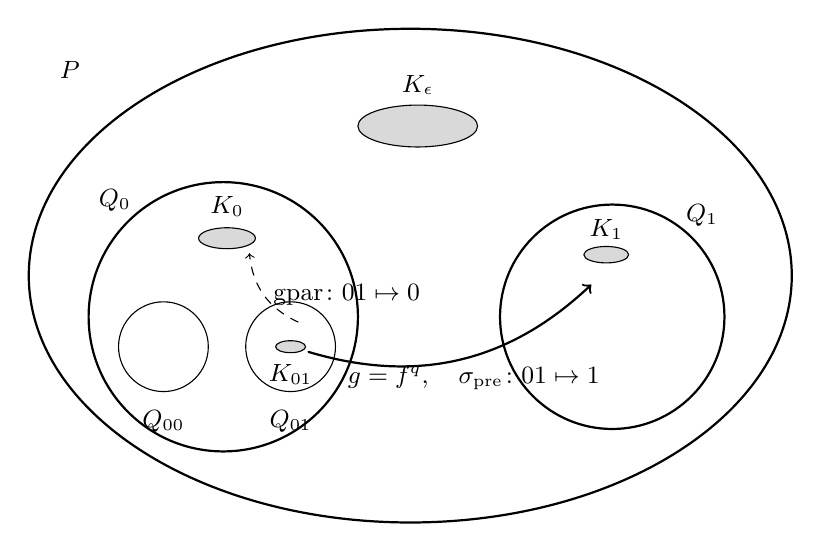
\begin{tikzpicture}[line cap=round, line join=round, scale=0.95,
  every node/.style={font=\small}]
 \draw[thick] (0,0) ellipse (5.1 and 3.3);
 \node at (-4.55,2.75) {$P$};
 \draw[thick] (-2.5,-0.55) circle (1.8);
 \node at (-3.95,1.0) {$Q_0$};
 \draw[thick] (2.7,-0.55) circle (1.5);
 \node at (3.9,0.8) {$Q_1$};
 \filldraw[fill=black!15] (0.1,2.0) ellipse (0.8 and 0.28);
 \node at (0.1,2.55) {$K_\epsilon$};
 \draw (-3.3,-0.95) circle (0.6);
 \node at (-3.3,-1.95) {$Q_{00}$};
 \draw (-1.6,-0.95) circle (0.6);
 \node at (-1.6,-1.95) {$Q_{01}$};
 \filldraw[fill=black!15] (-2.45,0.5) ellipse (0.38 and 0.14);
 \node at (-2.45,0.92) {$K_0$};
 \filldraw[fill=black!15] (-1.6,-0.95) ellipse (0.2 and 0.08);
 \node at (-1.6,-1.32) {$K_{01}$};
 \filldraw[fill=black!15] (2.62,0.28) ellipse (0.3 and 0.11);
 \node at (2.62,0.62) {$K_1$};
 \draw[->, dashed] (-1.5,-0.62) to[bend left=30]
   node[right, pos=0.5]{$\gpar\colon 01\mapsto 0$} (-2.15,0.3);
 \draw[->, thick] (-1.36,-1.02) to[bend right=30]
   node[below, pos=0.55]{$g=f^q,\quad \spre\colon 01\mapsto 1$}
   (2.42,-0.12);
\end{tikzpicture}
\caption{The two parent maps at address $01$.  Geometrically
$Q_{01}=\phi_0(Q_1)\subset Q_0$, so deleting the \emph{last} symbol
moves to the surrounding cylinder and its fiber,
$K_{01}\rightsquigarrow K_0$ (dashed arrow; containment, no dynamics).
Dynamically $g(Q_{01})=Q_1$ and $g(K_{01})=K_1$, so deleting the
\emph{first} symbol is the actual transition by $f^q$ (solid arrow).
The root $K_\epsilon$ sits in the first-level gap
$P\setminus(Q_0\cup Q_1)$; the fiber $K_0=\phi_0(K_\epsilon)$ sits in
the gap of $Q_0$ between its children $Q_{00},Q_{01}$.}
\label{fig:two-parents}
\end{figure}

\begin{remark}[Two parent maps]
\label{rem:two-parents}
The package carries two structurally different parent arrows
(\cref{fig:two-parents}):
\begin{equation}
 \gpar(wa)=w,
 \qquad
 \spre(a\alpha)=\alpha .
\label{eq:two-parents}
\end{equation}
The \emph{geometric parent} $\gpar$ deletes the \emph{last} symbol of a
nonempty finite word.  It is realized by cylinder inclusion,
$Q_{wa}\subset Q_w$, and by \emph{no} dynamical map: there is in
general no iterate of $f$ carrying $K_{wa}$ onto $K_w$.  It has no
action on ends, which have no last symbol.

The \emph{dynamical parent} $\spre$ deletes the \emph{first} symbol.
It is defined on all non-root finite addresses and on \emph{all} ends,
and it is realized by the exact two-branch covering of
\cref{thm:partial-shift}, with transition time $q$ and the deleted
symbol as inverse sheet.  Concretely, at address $01$:
$\gpar(01)=0$ because $Q_{01}=\phi_0(Q_1)\subset Q_0$, while
$\spre(01)=1$ because $g(K_{01})=K_1$.  The two arrows agree on no
address of length $\ge2$ in general, and conflating them collapses the
distinction between nesting depth and dynamical time.  Both are
retained as separate typed data.
\end{remark}

\begin{remark}[The root arrow is separate data]
\label{rem:root-arrow}
The dynamical parent $\spre$ is undefined at the empty word.  The root
has its own transition, coming from the terminal cycle of
\cref{prop:cycle-exclusion}:
\begin{equation}
 \troot\colon\quad
 g(\rootK)=f^q(\rootK)=\Kcyc_{\,q\bmod p}.
\label{eq:root-arrow}
\end{equation}
This arrow lands on a component of the terminal cycle; its target is
indexed by the cycle rather than by an address, and no positional claim
about $\Kcyc_{\,q\bmod p}$ relative to $\HB$ is made beyond
\cref{prop:cycle-exclusion}.  It is \emph{not} an extension of $\spre$,
and no assertion is made that the image escapes $\HB$ permanently
(\cref{nonclaims:main}\ref{N1}).  Keeping $\troot$ as a separate typed
arrow, rather than force-fitting it into the shift, is precisely what
makes the package close up without a circular hypothesis.
\end{remark}

\subsection{Naturality under root enlargement}

The virtual program enlarges its root package.  The compactification is
functorial under exactly the enlargements that stay in the gap.  For a
compact connected $R$ with
$\rootK\subset R\subset P\setminus(Q_0\cup Q_1)$, write
\[
 \HB(R)
 =
 \bigcup_{w\in\Words}\phi_w(R)
 \ \cup\
 \bigcup_{\omega\in\Ends}E_\omega
\]
for the compactum with root $R$; thus $\HB=\HB(\rootK)$.

\begin{theorem}[Root-gap enlargement naturality]
\label{thm:gap-enlargement}
Let
\begin{equation}
 \rootK\subset S\subset S^+
 \subset P\setminus(Q_0\cup Q_1)
\label{eq:gap-chain}
\end{equation}
be compact connected roots.  Then for each $R\in\{S,S^+\}$:
\begin{enumerate}[label=\textup{(\roman*)}]
 \item all separations of \cref{lem:cylinder-separations}, the
  conclusion of \cref{lem:label-limit}, and conclusions
  \ref{cpt:address}, \ref{cpt:components}, \ref{cpt:usc},
  \ref{cpt:action} of \cref{thm:compactification} hold for $\HB(R)$;
  $\HB(R)$ is compact and every fiber is a nonempty continuum;
 \item the component quotient and partial-shift theorems
  (\cref{thm:quotient,thm:partial-shift}) hold for $\HB(R)$, with root
  fiber $R$ in place of $\rootK$;
 \item membership in the filled Julia set is exactly
  \[
   \HB(R)\subset K(f)
   \iff
   R\subset K(f),
  \]
  and under \ref{H3} the same equivalence holds with $J(f)$;
 \item the inclusions $\phi_w(S)\subset\phi_w(S^+)$ commute with $g$
  at every finite word, and the end fibers are unchanged.
\end{enumerate}
\end{theorem}

\begin{proof}
(i)--(ii)  The proofs of the listed conclusions use the root only
through compactness, connectedness, containment in $P$, and
disjointness from $Q_0\cup Q_1$---the consequences of
\eqref{eq:root-gap} actually invoked there---all of which hold for $S$
and $S^+$ by \eqref{eq:gap-chain}.  The only step of
\cref{thm:compactification}\ref{cpt:compact} not covered is the
containment of the fibers in $K(f)$, which used
$\rootK\subset K(f)$ and is treated separately in (iii).  The quotient
and partial-shift proofs use only the separations, the label-limit
lemma, compactness, and \ref{H1}--\ref{H2}, so they persist verbatim.

(iii)  If $R\subset K(f)$, complete invariance of $K(f)$ gives
$\phi_w(R)\subset f^{-q|w|}(K(f))=K(f)$, and the end fibers lie in
$K(f)$ by the bounded-orbit argument of
\cref{thm:compactification}\ref{cpt:compact}; hence
$\HB(R)\subset K(f)$.  Conversely $R$ is the root fiber of $\HB(R)$,
so $\HB(R)\subset K(f)$ forces $R\subset K(f)$.  Under \ref{H3},
$K(f)=J(f)$.

(iv)  Injectivity of $\phi_w$ gives
$\phi_w(S)\subset\phi_w(S^+)$, and $g\circ\phi_a=\mathrm{id}$ gives the
commuting squares.  The end fibers \eqref{eq:end-fibers} depend only on
$P,Q_0,Q_1$.
\end{proof}

\begin{remark}[Three levels of enlargement, and the root arrow]
\label{rem:enlargement-scope}
\Cref{thm:gap-enlargement} is the \emph{topological} level: it needs
only a compact connected root in the gap, and it does not assert that
$S$ or $S^+$ is full, contained in $J(f)$, dynamically protected,
access-complete, or admissible as an analytic virtual carrier; those
properties are separate audits.  The \emph{fullness/cell} level
requires a full root compactly contained in the open gap component
$G_0$ and is treated in \cref{cor:full-root}.  The \emph{Julia} level
is the equivalence (iii).  Finally, the root arrow
\eqref{eq:root-arrow} refers to the terminal cycle of the original
root $\rootK$; for an enlarged root $R$ the image $g(R)$ carries no
terminal-cycle identification, and any dynamical meaning of the
enlarged root arrow requires a separate audit.
\end{remark}

\section{Fullness, the end compactum, gap cells, and replacement}
\label{sec:fullness}

\subsection{Full fibers and connected complement}

\begin{theorem}[Full fibers and nonseparation]
\label{thm:full-nonseparating}
Every fiber $K_w$ and $E_\omega$ of \cref{thm:compactification} is a
full continuum, and $\Chat\setminus\HB$ is connected.  Moreover, for
every Jordan domain $U$ with $P\Subset U$, the relative complement
$U\setminus\HB$ is connected.
\end{theorem}

\begin{proof}
The root $\rootK$ is full \cite{DH85}.  Each
$\phi_w\colon P\to Q_w$ is an orientation-preserving homeomorphism of
closed Jordan disks, so $K_w=\phi_w(\rootK)$ is full by
\cref{lem:jordan-transport}\ref{jt:full}.  For an end,
\[
 \Chat\setminus E_\omega
 =
 \bigcup_{m\ge1}
 \bigl(\Chat\setminus Q_{\omega|m}\bigr)
\]
is an increasing union of connected sets containing $\infty$, hence
connected; so $E_\omega$ is full.

For $m\ge0$ define the approximants
\begin{equation}
 \HB^{(m)}
 =
 \bigcup_{|u|<m}K_u
 \ \cup\
 \bigcup_{|w|=m}Q_w .
\label{eq:approximants}
\end{equation}
Each term is full, and the terms of $\HB^{(m)}$ are pairwise disjoint:
equal-depth cylinders are disjoint
(\cref{lem:cylinder-separations}\ref{sep:incomparable}), distinct finite
fibers are disjoint (\ref{sep:all}), and for $|u|<m=|w|$ the word $u$ is
either incomparable to $w$ (disjoint cylinders) or a strict prefix of
$w$ (then $K_u\cap Q_w=\varnothing$ by \ref{sep:gap}).  The sets
\eqref{eq:approximants} decrease in $m$: each $K_u$ with $|u|=m$ lies in
$Q_u$, and each $Q_w$ with $|w|=m+1$ lies in $Q_{w|m}$.

Their intersection is exactly $\HB$.  Indeed $\HB\subset\HB^{(m)}$ for
every $m$ (a fiber with address of length $\ge m$ or an end fiber lies
in its depth-$m$ cylinder).  Conversely, let
$x\in\bigcap_m\HB^{(m)}$.  If $x$ lies in some finite fiber $K_u$ we are
done.  Otherwise, for every $m$ there is a unique word $w_m$ of length
$m$ with $x\in Q_{w_m}$ (uniqueness by disjointness of equal-depth
cylinders), and $x\in Q_{w_{m+1}}\subset Q_{w_{m+1}|m}$ forces
$w_{m+1}|m=w_m$.  The words $w_m$ therefore converge to an end $\omega$
with $x\in\bigcap_mQ_{\omega|m}=E_\omega$.

\Cref{lem:nested-full-packets} applied to the decreasing packets
\eqref{eq:approximants} proves that $\Chat\setminus\HB$ is connected;
its localized clause, applied with the exterior full continuum
$\Chat\setminus U$ adjoined to each packet, proves that
$U\setminus\HB$ is connected.
\end{proof}

\subsection{The end compactum}

\begin{corollary}[Cantor-indexed end compactum]
\label{cor:end-compactum}
Let
\[
 \HE=\bigcup_{\omega\in\Ends}E_\omega .
\]
Then
\begin{equation}
 \HE=\bigcap_{m\ge1}\ \bigcup_{|w|=m}Q_w ,
\label{eq:end-compactum}
\end{equation}
$\HE$ is compact, its connected components are precisely the end fibers
$E_\omega$, and $\Chat\setminus\HE$ is connected.  The component
quotient restricts to a continuous closed surjection
$\HE\to\Ends=\{0,1\}^{\N}$, so the component space of $\HE$ is the
Cantor space, and
\[
 g\colon\HE\longrightarrow\HE
\]
is a trivial two-sheeted covering of $\HE$ over itself, semiconjugate
under the quotient to the one-sided binary shift, realized by the two
univalent branches $\phi_0,\phi_1$ of $f^{-q}$.
\end{corollary}

\begin{proof}
For \eqref{eq:end-compactum}: every $E_\omega$ lies in $Q_{\omega|m}$
for all $m$, giving one inclusion.  Conversely, a point $x$ of the
right-hand side lies, for every $m$, in a unique depth-$m$ cylinder
$Q_{w_m}$, and uniqueness forces $w_{m+1}|m=w_m$ as in
\cref{thm:full-nonseparating}; hence $x\in E_\omega$ for
$\omega=\lim w_m$.  No finite fiber meets the right-hand side: for
$m>|u|$, $K_u$ misses every depth-$m$ cylinder
(\cref{lem:cylinder-separations}\ref{sep:gap} and
\ref{sep:incomparable}).  Thus \eqref{eq:end-compactum} holds, and
$\HE$ is an intersection of compacta, hence compact.

The levels $\bigcup_{|w|=m}Q_w$ are finite unions of pairwise disjoint
full continua and decrease in $m$, so \cref{lem:nested-full-packets}
makes $\Chat\setminus\HE$ connected.  Components: the sets
$\HE\cap Q_u$ are clopen in $\HE$ (they are the restrictions of the
clopen sets $\HB[u]$ of \cref{thm:compactification}), and the argument
of \cref{thm:compactification}\ref{cpt:components} applies verbatim
with only end addresses present.  The quotient statement restricts
\cref{thm:quotient}; $\Ends\subset\OmB$ is closed, and the restricted
map is again a continuous closed surjection.  Finally
$\phi_a(\HE)=\HE\cap Q_a$ and $g(E_{a\omega})=E_\omega$ give the
two-sheeted covering of $\HE$ over itself and the semiconjugacy to the
full one-sided shift, exactly as in \cref{thm:partial-shift}; here no
root is removed, since $\spre$ is total on ends.
\end{proof}

\begin{remark}
$\HE$ is the statement most directly comparable to a ``Cantor family of
continua'': a compact nonseparating union of full continua whose
component space is $\{0,1\}^{\N}$ and on which the binary shift is
realized by two actual univalent inverse branches.  It does not
identify the $E_\omega$ as small Julia sets
(\cref{nonclaims:main}\ref{N2}); it realizes exactly the topological
and dynamical skeleton.
\end{remark}

\subsection{The gap-cell atlas}

Recall $G_0$, the component of
$\operatorname{int}P\setminus(Q_0\cup Q_1)$ containing $\rootK$
(\cref{hyp:standing}\ref{H4}).  By
\cref{lem:full-jordan-neighborhood} choose once and for all a closed
Jordan disk $D$ with
\begin{equation}
 \rootK\subset\operatorname{int}D\subset D\Subset G_0,
\label{eq:root-cell}
\end{equation}
and put $D_w=\phi_w(D)$.

\begin{theorem}[Gap-cell atlas]
\label{thm:gap-cells}
The closed Jordan cells $D_w$ are pairwise disjoint---including for
ancestor--descendant pairs---and satisfy
\begin{align}
 K_w\subset\operatorname{int}D_w,
 \qquad
 &D_w\Subset
 \operatorname{int}Q_w\setminus(Q_{w0}\cup Q_{w1}),
\label{eq:cell-location}\\
 D_w\cap\HB=K_w,
 \qquad
 &g(D_{aw})=D_w .
\label{eq:cell-trace}
\end{align}
If $S_w\Subset\operatorname{int}D_w$ is compact and connected, then
\begin{equation}
 \Fill(S_w)\Subset\operatorname{int}D_w .
\label{eq:cell-fill}
\end{equation}
\end{theorem}

\begin{proof}
By \eqref{eq:root-cell} and \ref{H2}, $\phi_w$ carries
$\operatorname{int}P$ to $\operatorname{int}Q_w$, $Q_a$ to $Q_{wa}$, and
$D$ to $D_w$, which proves \eqref{eq:cell-location}.  For disjointness:
incomparable words have disjoint cylinders containing their cells; and
if $v=uat$ is a strict descendant of $u$, then $D_v$ lies in the child
cylinder $Q_{ua}$ while $D_u$ misses both children of $Q_u$ by
\eqref{eq:cell-location}.

First identity of \eqref{eq:cell-trace}: fibers with address strictly
extending $w$ lie in the children $Q_{w0}\cup Q_{w1}$, which $D_w$
misses; fibers with address incomparable to $w$ miss $Q_w\supset D_w$;
fibers $K_u$ with $u$ a strict prefix of $w$ miss
$Q_{w|_{|u|+1}}\supset D_w$ by
\cref{lem:cylinder-separations}\ref{sep:gap}; end fibers extending $w$
lie in a child of $Q_w$.  What remains is
$K_w\subset\operatorname{int}D_w$.  The second identity follows from
$g\circ\phi_a=\mathrm{id}$.

For \eqref{eq:cell-fill}: a collar of $\partial D_w$ together with the
exterior of $D_w$ is a connected subset of the unbounded component of
$\C\setminus S_w$; every bounded complementary component of $S_w$ is
therefore contained away from that collar, inside
$\operatorname{int}D_w$.
\end{proof}

\subsection{Cellwise replacement at arbitrary addresses}

The next theorem removes the finiteness restriction of the packet
replacement used in Draft~I.  Replacement may occur at \emph{every}
finite address simultaneously; finiteness is required only where the
connector construction of \cref{sec:carrier} actually uses it.

\begin{theorem}[Cellwise packet replacement at arbitrary addresses]
\label{thm:cellwise-replacement}
Let $F\subset\Words$ be an arbitrary---possibly infinite---set of
finite addresses, and for each $w\in F$ let $L_w$ be a compact
connected set with
\begin{equation}
 K_w\subset L_w\Subset\operatorname{int}D_w .
\label{eq:replacement-data}
\end{equation}
Put $\widetilde K_w=L_w$ for $w\in F$ and $\widetilde K_w=K_w$
otherwise, and
\begin{equation}
 \widetilde{\mathcal H}
 =
 \bigcup_{w\in\Words}\widetilde K_w
 \ \cup\
 \bigcup_{\omega\in\Ends}E_\omega .
\label{eq:replaced}
\end{equation}
Then:
\begin{enumerate}[label=\textup{(\roman*)}]
 \item \label{rep:top} $\widetilde{\mathcal H}$ is compact; its
  connected components are exactly the sets $\widetilde K_w$
  ($w\in\Words$) and $E_\omega$ ($\omega\in\Ends$); the realization
  $\alpha\mapsto\widetilde{\mathrm{fib}}(\alpha)$ is upper
  semicontinuous; and the component projection
  $\widetilde\pi\colon\widetilde{\mathcal H}\to\OmB$ is a continuous
  closed surjection.
 \item \label{rep:full} If in addition every $L_w$ ($w\in F$) is full,
  then $\Chat\setminus\widetilde{\mathcal H}$ is connected, and for
  every Jordan domain $U$ with $P\Subset U$ the relative complement
  $U\setminus\widetilde{\mathcal H}$ is connected.
\end{enumerate}
The containment $K_w\subset L_w$ is used nowhere in the proof of
\ref{rep:top}; it records the enlargement semantics and may be dropped.
\end{theorem}

\begin{proof}
Define the modified approximants
\begin{equation}
 \widetilde{\mathcal H}^{(m)}
 =
 \bigcup_{|u|<m}\widetilde K_u
 \ \cup\
 \bigcup_{|w|=m}Q_w .
\label{eq:mod-approximants}
\end{equation}
At each fixed $m$ this is a \emph{finite} union---fewer than $2^m$
packets and exactly $2^m$ cylinders---regardless of the cardinality of
$F$.  The terms are pairwise disjoint: distinct packets lie in the
pairwise disjoint cells $D_u$ (both $K_u$ and $L_u$ lie in
$\operatorname{int}D_u$ by \eqref{eq:cell-location} and
\eqref{eq:replacement-data}); a packet $\widetilde K_u$ with $|u|<m$
and a cylinder $Q_w$ with $|w|=m$ are disjoint because either $u$ is a
strict prefix of $w$, in which case $Q_w$ lies in a child of $Q_u$,
which $D_u\supset\widetilde K_u$ misses by \eqref{eq:cell-location}, or
$u$ and $w$ are incomparable, in which case already
$Q_u\cap Q_w=\varnothing$.  The sets \eqref{eq:mod-approximants}
decrease in $m$: each $\widetilde K_u$ with $|u|=m$ lies in
$\operatorname{int}D_u\subset Q_u$, and each depth-$(m{+}1)$ cylinder
lies in its parent.

The intersection of the modified approximants is exactly
$\widetilde{\mathcal H}$: one inclusion is clear as before, and if
$x\in\bigcap_m\widetilde{\mathcal H}^{(m)}$ lies in no packet
$\widetilde K_u$, then at every depth it lies in a unique cylinder,
the words nest, and $x$ lies in the corresponding end fiber.
Compactness of $\widetilde{\mathcal H}$ follows, each approximant being
compact.

For the component structure, upper semicontinuity, and the quotient in
\ref{rep:top}, the arguments of
\cref{thm:compactification,thm:quotient} apply verbatim once their two
inputs are re-verified for the modified fibers.  First, the
separations: distinct packets lie in disjoint cells; a packet
$\widetilde K_u$ misses every cylinder $Q_v$ with $v$ strictly
extending $u$ (it lies in $D_u$, which misses the children of $Q_u$)
and every cylinder incomparable to $u$; hence distinct modified fibers
are pairwise disjoint, and the clopen sets
$\widetilde{\mathcal H}\cap Q_u$ again consist exactly of the modified
fibers with address extending $u$.  Second, the label-limit lemma: if
$\alpha_j\to\alpha$ and
$x_j\in\widetilde{\mathrm{fib}}(\alpha_j)\to x$, then for finite
$\alpha$ the labels are eventually constant and
$\widetilde K_\alpha$ is closed, while for an end $\alpha$ every
modified fiber with address extending $\alpha|m$ lies in
$Q_{\alpha|m}$ (packets via
$\widetilde K_v\subset D_v\subset Q_v\subset Q_{\alpha|m}$), so
$x\in E_\alpha$.  With these two inputs, the clopen-partition
components argument, the closed-graph upper semicontinuity, and the
continuity-closedness of the component projection repeat word for
word.

For \ref{rep:full}, every term of \eqref{eq:mod-approximants} is now
full ($L_w$ by hypothesis, $K_u$ and $Q_w$ as before), so
\cref{lem:nested-full-packets} and its localized clause apply to the
decreasing packets, with the exterior continuum $\Chat\setminus U$
adjoined for the relative statement.
\end{proof}

\begin{remark}
\label{rem:replacement-scope}
No uniform diameter estimate, no coherence between the $L_w$ at
different addresses, and no dynamical compatibility is required in
\cref{thm:cellwise-replacement}; correspondingly, no equivariance is
asserted for the replaced package---$g(L_{aw})$ need not equal $L_w$.
Equivariance returns exactly for coherent families
$L_w=\phi_w(S)$, which is the content of \cref{cor:full-root}.  For
nonfull replacements, part \ref{rep:top} survives while part
\ref{rep:full} genuinely fails in general
(Appendix~\ref{app:tests}, \cref{test:nonfull}).
\end{remark}

\subsection{Full root-gap naturality}

\begin{corollary}[Full root-gap naturality]
\label{cor:full-root}
Let $S$ be a nondegenerate full continuum with
\[
 \rootK\subset S\Subset G_0 ,
\]
and put $S_w=\phi_w(S)$.  Then the full package holds for the root $S$:
\begin{enumerate}[label=\textup{(\roman*)}]
 \item $\HB(S)=\bigcup_wS_w\cup\bigcup_\omega E_\omega$ is compact,
  its components are exactly the $S_w$ and $E_\omega$, the component
  projection onto $\OmB$ is a continuous closed surjection, and
  $g\colon\HB(S)\setminus S\to\HB(S)$ is a trivial two-sheeted covering
  with $g(S_{aw})=S_w$;
 \item every $S_w$ is full, $\Chat\setminus\HB(S)$ is connected, and
  $U\setminus\HB(S)$ is connected for every Jordan domain $U$ with
  $P\Subset U$;
 \item there is a gap-cell atlas for $S$: a closed Jordan disk $D_S$
  with $S\subset\operatorname{int}D_S\subset D_S\Subset G_0$ whose
  transported cells $D_{S,w}=\phi_w(D_S)$ satisfy all conclusions of
  \cref{thm:gap-cells} with $S_w$ in place of $K_w$;
 \item $\HB(S)\subset K(f)$ if and only if $S\subset K(f)$; under
  \ref{H3} the same holds with $J(f)$.
\end{enumerate}
\end{corollary}

\begin{proof}
The root $S$ is compact, connected, nondegenerate, full, and satisfies
the gap relation
$S\subset G_0\subset\operatorname{int}P\setminus(Q_0\cup Q_1)$; that
is, $S$ satisfies \ref{H4} verbatim.  Part (i) is
\cref{thm:gap-enlargement}(i)--(ii) with $R=S$, together with
$g\circ\phi_{aw}=\phi_w$ for the displayed equivariance.  Part (ii)
reruns the proof of \cref{thm:full-nonseparating} with root $S$: that
proof uses only fullness of the root, the separations, and \ref{H2},
all available.  Part (iii) reruns \cref{thm:gap-cells}:
\cref{lem:full-jordan-neighborhood} applies to the nondegenerate full
continuum $S\Subset G_0$ and produces $D_S$, and the proof of
\cref{thm:gap-cells} uses only \eqref{eq:root-cell}-type containment,
\ref{H2}, and the separations.  Part (iv) is
\cref{thm:gap-enlargement}(iii).
\end{proof}

\section{The finite protected carrier}
\label{sec:carrier}

The final theorem combines the package with the connector technology of
\cref{sec:connector}.  It is the dynamical payoff: finitely many
protected accesses at the root transport to finitely many selected
fibers, and a connected full carrier realizes them simultaneously while
meeting the compactum in exactly the selected fibers.  Here finiteness
is genuinely used---the connector is a finite tree---in contrast to the
replacement theorem, which is not so restricted.

\begin{lemma}[Proper protected impressions leave a port]
\label{lem:impression-port}
Let $K\Subset\operatorname{int}D$ be a nondegenerate full continuum in a
closed Jordan disk $D$ and let
$P_{\mathrm{prot}}\subsetneq\partial K$ be compact, possibly empty.
There are $x\in\partial K\setminus P_{\mathrm{prot}}$ and a Jordan arc
$\alpha$ from $x$ to $\partial D$, otherwise in
$\operatorname{int}D\setminus K$.  Moreover, finitely many crosscut
chains of $\Chat\setminus K$ whose impressions have union contained in
$P_{\mathrm{prot}}$ can be truncated so that, writing $S$ for the
connected union of $K$ with the truncated relative collar tails,
\begin{equation}
 \alpha\cap\Fill(S)=\{x\}.
\label{eq:port-clearance}
\end{equation}
\end{lemma}

\begin{proof}
If $P_{\mathrm{prot}}=\varnothing$, choose any $y\in\partial K$ and
skip the distance argument below (there are then no chains to
truncate, $S=K$, and only the port construction is needed).  Otherwise
choose $y\in\partial K\setminus P_{\mathrm{prot}}$ and put
$\delta=\operatorname{dist}(y,P_{\mathrm{prot}})>0$.  Choose
$z\in\operatorname{int}D\setminus K$ with $|z-y|<\delta/4$, and let
$x\in K$ minimize distance to $z$.  The segment $(x,z]$ misses $K$, and
$|x-y|\le2|z-y|<\delta/2$, so
$x\notin P_{\mathrm{prot}}$.  The complement of the full continuum $K$
in $\Chat$ is an open connected, hence arcwise connected, set; join $z$
to the exterior of $D$, take a simple subarc of the concatenation
starting at $x$, and stop at its first hit on $\partial D$.  This is
$\alpha$.

The compact arc $\alpha$ misses the compact set $P_{\mathrm{prot}}$ at
positive distance.  For each chain, the nested compact sets
$\overline{D_n}$ have intersection equal to the impression, which lies
in $P_{\mathrm{prot}}$; hence sufficiently deep relative tails lie in
prescribed neighborhoods of the impressions chosen to miss $\alpha$.
Truncate each chain there.  Finally, extending $\alpha$ beyond
$\partial D$ to $\infty$ shows that every point of $\alpha$ except $x$
lies in the unbounded component of $\C\setminus S$, which proves
\eqref{eq:port-clearance}.
\end{proof}

\begin{theorem}[Finite direct-decoration protected carrier]
\label{thm:protected-carrier}
Fix a nonempty finite set $F\subset\Words$ of addresses and finitely
many (possibly zero) crosscut chains of $\Chat\setminus\rootK$ (the
\emph{protected root chains}) whose relative terminal collar tails are
pairwise disjoint and whose total impression is a proper compact subset
$P_{\mathrm{prot}}\subsetneq\partial\rootK$.  Let $U$ be a Jordan
domain with $P\Subset U$.  Then the chains can be truncated and
transported by the inverse branches $\phi_w$ ($w\in F$), and there
exist a free port point $x_w\in\partial K_w$ and a port arc $\alpha_w$
for each $w\in F$, such that:
\begin{enumerate}[label=\textup{(\roman*)}]
 \item \label{car:packets} the transported packet fullifications
  $L_w=\Fill\bigl(K_w\cup(\text{transported relative collar
  tails})\bigr)$ satisfy $K_w\subset L_w\Subset\operatorname{int}D_w$,
  so they lie in the pairwise disjoint gap cells of
  \cref{thm:gap-cells};
 \item \label{car:carrier} there is a compact connected full carrier
  $H\Subset U$ containing every selected fiber $K_w$ ($w\in F$) with
  singleton attachment trace
  $\overline{H\setminus K_w}\cap K_w=\{x_w\}$, and meeting the
  compactum in exactly the selected fibers:
  \begin{equation}
   H\cap\HB=\bigcup_{w\in F}K_w ;
  \label{eq:exact-trace}
  \end{equation}
 \item \label{car:survival} every transported protected chain survives
  as a prime-end chain of $\Chat\setminus H$, and the survival map is
  injective and preserves the cyclic order of the transported family
  in $\Chat\setminus H$;
 \item \label{car:no-lc} no local connectivity of any fiber is assumed
  or concluded.
\end{enumerate}
\end{theorem}

\begin{proof}
\emph{Step 1: root port and truncation.}
Apply \cref{lem:impression-port} with $K=\rootK$, the cell $D$ of
\eqref{eq:root-cell}, and $P_{\mathrm{prot}}$ (the lemma covers
$P_{\mathrm{prot}}=\varnothing$): this yields a free point
$x\in\partial\rootK\setminus P_{\mathrm{prot}}$, an arc $\alpha$ from
$x$ to $\partial D$ otherwise in
$\operatorname{int}D\setminus\rootK$, and truncations of the chains
such that, for the connected union $S$ of $\rootK$ with the truncated
relative collar tails, \eqref{eq:port-clearance} holds.  Truncating
further if necessary, $S\Subset\operatorname{int}D$: the sets
$\overline{D_n}$ shrink to impressions on
$\partial\rootK\subset\operatorname{int}D$.  The truncated relative
tails are pairwise disjoint: by the null-chain condition
\eqref{eq:null-chain}, each truncated relative tail lies in the open
terminal collar of its own chain, and those collars contain the
pairwise disjoint original relative terminal tails of the
hypothesis---so distinct chains' truncated tails lie in disjoint sets.

\emph{Step 2: transport.}
For $w\in F$ put
\[
 S_w=\phi_w(S),\qquad
 L_w=\Fill(S_w),\qquad
 x_w=\phi_w(x),\qquad
 \alpha_w=\phi_w(\alpha).
\]
Each $\phi_w$ restricts to an orientation-preserving homeomorphism of
closed Jordan disks $D\to D_w$ (\ref{H2}, \cref{thm:gap-cells}).  By
the pointed Schoenflies transport
(\cref{lem:jordan-transport}\ref{jt:fill}), it commutes with $\Fill$
on compact subsets of $D$, carries crosscut chains of
$\Chat\setminus\rootK$ to crosscut chains of $\Chat\setminus K_w$
preserving selected sides, the null-chain condition, and cyclic order,
and transports \eqref{eq:port-clearance} to
\begin{equation}
 \alpha_w\cap L_w=\{x_w\}.
\label{eq:transported-port}
\end{equation}
Since $S\Subset\operatorname{int}D$ is compact and connected,
\cref{thm:gap-cells}\eqref{eq:cell-fill} gives
$L_w=\Fill(S_w)\Subset\operatorname{int}D_w$, proving
\ref{car:packets}.  The arc $\alpha_w$ runs from $x_w$ to
$\partial D_w$, otherwise in $\operatorname{int}D_w\setminus L_w$.

\emph{Step 3: one free component.}
The data \eqref{eq:replacement-data} hold for the finite family
$\{L_w\}_{w\in F}$ with every $L_w$ full, so
\cref{thm:cellwise-replacement}\ref{rep:full} applies:
$U\setminus\widetilde{\mathcal H}$ is connected, where
$\widetilde{\mathcal H}$ is the replaced compactum
\eqref{eq:replaced}.  Set the connector inventory of
\cref{sec:connector} as follows: atoms $A_w:=K_w$ ($w\in F$); protected
collars: the transported truncated relative collar tails, which are
pairwise disjoint---within one fiber by Step~1 and injectivity of
$\phi_w$, across fibers because they lie in the pairwise disjoint
cells $D_w$; forbidden set
$Z:=\HB\setminus\bigcup_{w\in F}K_w$ (every unselected finite fiber
and every end fiber), which is compact because the selected fibers are
clopen in $\HB$.  Then the frozen set $Q$ of \eqref{eq:free-domain}
satisfies $Q\subset\widetilde{\mathcal H}$: atoms and relative collar
tails lie in the packets $L_w$, and
$Z\subset\widetilde{\mathcal H}$.  Hence
\[
 U\setminus\widetilde{\mathcal H}\ \subset\
 \Omega_{\mathrm{free}}=U\setminus Q,
\]
and the connected set $U\setminus\widetilde{\mathcal H}$ lies in one
component $\Omega_0$ of $\Omega_{\mathrm{free}}$.

The port interiors lie in that component: by
\eqref{eq:transported-port} and \eqref{eq:cell-trace},
\[
 \alpha_w((0,1])\ \subset\
 \bigl(\operatorname{int}D_w\setminus L_w\bigr)
 \cup\partial D_w
 \ \subset\ U\setminus\widetilde{\mathcal H},
\]
because $D_w\cap\widetilde{\mathcal H}=L_w$ (the cell meets the
replaced compactum exactly in its own packet, by \eqref{eq:cell-trace}
and disjointness of the cells) and $\partial D_w$ misses
$\widetilde{\mathcal H}$.  Also
$\alpha_w\cap K_w\subset\alpha_w\cap L_w=\{x_w\}$ with
$x_w\in\partial K_w$ free: $x=\phi_w^{-1}(x_w)$ is not in
$P_{\mathrm{prot}}$ and hence $x_w$ is not an impression of a
transported chain.  The arcs $\alpha_w$ are pairwise disjoint, lying
in the pairwise disjoint closed cells $D_w$.  Thus $\Omega_0$ has
simultaneous singleton ports to every atom.

\emph{Step 4: certificate and carrier.}
\Cref{thm:free-component} yields a protected ribbon-routing
certificate for the atoms $K_w$, protected collars, and forbidden set
$Z$, with connector tree $T_{\mathfrak R}$ satisfying
\eqref{eq:tree-incidence}, and \cref{thm:connector} realizes it: a
compact connected full carrier $H=H_{\mathfrak R}\Subset U$ containing
every $K_w$ with singleton attachment traces $\{x_w\}$, missing $Z$,
with every transported chain surviving as a prime-end chain of
$\Chat\setminus H$, injectively and in the cyclic order of the
transported family.  For the exact trace \eqref{eq:exact-trace}:
$H\supset\bigcup_{w\in F}K_w$ by construction, and
$H\setminus\bigcup_{w\in F}K_w=T_{\mathfrak R}\setminus\{x_w:w\in F\}$
lies in $\Omega_{\mathrm{free}}\cup\{\alpha_w(1)\}$, which misses
$Z\cup\bigcup_{w\in F}K_w=\HB$ except at the port points
$x_w\in K_w$ already counted; hence $H\cap\HB$ is exactly the union of
the selected fibers.  This proves \ref{car:carrier} and
\ref{car:survival}.  The arguments use crosscut chains and plane
topology only, never a boundary parametrization of any fiber, proving
\ref{car:no-lc}.
\end{proof}

\begin{remark}[Finite and direct-scale only]
\label{rem:carrier-scope}
\Cref{thm:protected-carrier} is finite and direct-scale only.  It does
not construct a second satellite portrait, an end-fiber return map, a
uniform incidence bound, or the future fjord, dam, and attachment data
of the virtual program (\cref{nonclaims:main}).  Selecting
\emph{infinitely} many fibers, or an end fiber, as atoms is not
covered by the theorem---the connector is a finite tree---although the
underlying packet compactum need not be finite
(\cref{thm:cellwise-replacement}).  \Cref{prop:fan-growth} shows that
the raw marking data grow without bound as the decoration depth
increases.
\end{remark}

\section{Scope and open problems}
\label{sec:scope}

\subsection{Why the remaining finiteness restriction is honest}

\begin{proposition}[Raw decoration-fan growth]
\label{prop:fan-growth}
The quadratic separator $Y^{(n-1)q+1}$ has exactly $2^n$ vertices, and
the decoration construction supplies a distinct pairwise-disjoint
univalent pullback $Q^v$ for every vertex \cite{KLDecorations08}.
Hence any marking that retains one distinct record for every source
$Q^v$ has at least $2^n$ entries and admits no universal cardinality
bound as $n$ varies.
\end{proposition}

\begin{proof}
The vertex count and the one-per-vertex pairwise disjoint pullbacks are
the source statements in \cite{KLDecorations08}.  Distinct disjoint
pullbacks require distinct marked records, so the cardinality is at
least $2^n$, which is unbounded in $n$.
\end{proof}

Thus a virtual construction over all scales requires either a uniformly
bounded proof-complete subset of the raw fan or a future-faithful
access compression; neither is constructed here
(\cref{nonclaims:main}\ref{N4}).  Note the division of labor after
\cref{thm:cellwise-replacement}: the packet \emph{compactum} supports
arbitrary, even infinite, cellwise modification, while the protected
\emph{connector} remains finite.

\subsection{What separates this model from the virtual package}

Dudko's virtual Julia sets are described as connected hulls of Cantor
families of small Julia sets carrying part of the critical orbit
\cite{Dudko25}.  The present package supplies the correctly typed
skeleton of such an object at one scale: address space, embedded
components, end fibers, the component quotient, both parent maps, root
arrow, cells, arbitrary cellwise replacement, and protected carrier.
What it does not supply is exactly what remains open:

\begin{enumerate}[label=(\alph*),leftmargin=2.4em]
 \item \emph{Identification of ends.}  The end fibers $E_\omega$ are
  nested puzzle intersections.  They have not been identified with
  small Julia sets, and no renormalization structure on them is
  claimed (\ref{N2}).
 \item \emph{Analytic end dynamics.}  The covering of
  \cref{thm:partial-shift} moves ends by deleting the first symbol; no
  first-return or self-return map \emph{on} a single end fiber is
  constructed (\ref{N3}).
 \item \emph{Portraits and markings.}  No second satellite portrait is
  constructed, and the transported prime-end data of
  \cref{thm:protected-carrier} concern finitely many chains at finitely
  many finite fibers only (\ref{N2}, \ref{N4}).
\end{enumerate}

The two open problems below record the missing constructions in the
typing of this paper.  They are stated for the checked sources
\cite{Dudko25,KKL26}; solving them would be a genuine advance
independent of this paper.

\begin{problem}[Virtual package realization]
\label{prob:virtual-package}
For each actual intermediate virtual scale, construct an actual compact
address space, nonempty compact connected components realizing it, and
exact polynomial branch, return, parent, sheet, critical-address,
escape, localization, and root-enlargement data---without using any
downstream width, compactness, rigidity, or MLC conclusion.  The present
paper solves the one-scale direct-decoration case; the virtual case at
deeper copies would pass through a disconnected intermediate satellite
object and currently assumes the virtual renormalization being
constructed.
\end{problem}

\begin{problem}[Marking transfer to the ends]
\label{prob:marking-transfer}
Transfer a second satellite portrait to actual puzzle or generalized
polynomial-like bases and actual iterates on the finite cylinders and
end fibers of \cref{thm:compactification}.  Prove equivariance under
\eqref{eq:equivariance}, analytic realization at every end, the declared
critical chronology, complete access and obstacle marking,
terminal-return compatibility (compatibility with the separate root
arrow $\troot$ of \cref{rem:root-arrow} and the terminal cycle of
\cref{prop:cycle-exclusion}; cf.\ \cref{nonclaims:main}\ref{N1}), and
naturality under every authorized root enlargement
(\cref{thm:gap-enlargement,cor:full-root}).
\end{problem}

\subsection{Relation to classical compactifications}

The address space \eqref{eq:address-space} is the standard end
compactification of the rooted binary tree, and nested-disk models of
it are classical.  The reader should therefore locate the contribution
precisely: it is not the topology of $\OmB$ but the statements proved
\emph{about the dynamical realization}---membership in $K(f)$ and, under
\ref{H3}, in $J(f)$; the exact component structure with its continuous
closed component quotient; upper semicontinuity; the exact two-branch
covering realization of the partial shift; the two-parent-map typing
with a separate root arrow; fullness and nonseparation with the
Cantor-indexed end compactum; the equivariant cell atlas with cellwise
replacement at arbitrary addresses; and the finite protected
carrier---together with the naturality of the compactification package
under the root enlargement that the virtual program actually performs
(\cref{thm:gap-enlargement,cor:full-root}).  Each of these is used as a
correctness criterion (a ``positive control'') against which a proposed
virtual package can be audited field by field, and
Appendix~\ref{app:tests} records the boundary cases that audit must
survive.

\subsection*{Machine-assistance disclosure}
Drafting, verification, and build tooling for this paper: Fae Build,
Anthropic Fable~5, and OpenAI GPT-5.6.  All mathematical claims and
their proofs are the author's responsibility.

\appendix

\section{Concordance with the program manuscript}
\label{app:concordance}

This paper extracts, makes self-contained, and strengthens a package
proved inside a larger program manuscript (\emph{A Marked-Width
Reduction of Mandelbrot Local Connectivity}, in preparation).  For the
reader with access to that manuscript, the concordance is:

\begin{center}
\begin{tabular}{ll}
\textbf{This paper} & \textbf{Program manuscript}\\[2pt]
\cref{thm:compactification} & Theorem 10.37\\
\cref{thm:quotient} & --- (new)\\
\cref{thm:partial-shift} & --- (new)\\
\cref{thm:gap-enlargement} & Theorem 10.38 (strengthened)\\
\cref{lem:nested-full-packets} & Lemma 10.39\\
\cref{thm:full-nonseparating} & Theorem 10.40\\
\cref{cor:end-compactum} & --- (new)\\
\cref{lem:full-jordan-neighborhood} & Lemma 10.41\\
\cref{thm:gap-cells} & Theorem 10.42\\
\cref{thm:cellwise-replacement} & Theorem 10.43 (finite case;
  arbitrary $F$ new)\\
\cref{cor:full-root} & --- (new)\\
\cref{lem:impression-port} & Lemma 10.44\\
\cref{thm:protected-carrier} & Theorem 10.45 (exact trace new)\\
\cref{thm:connector} & Theorem 10.4\\
\cref{thm:free-component} & Theorem 10.8\\
\cref{lem:disjoint-full-complement} & Lemma 10.10\\
\cref{lem:local-pullback} & --- (new)\\
\cref{prop:cycle-exclusion} & Proposition 10.31\\
\cref{prop:fan-growth} & Proposition 10.32
\end{tabular}
\end{center}

The manuscript numbering refers to its Section 10 (protected regulated
connectors and the direct-decoration pullback compactification).

\section{Adversarial boundary cases}
\label{app:tests}

Each test below names a boundary case an auditor should try, and where
the present proofs meet it.

\begin{test}[Closed pullbacks touching]
\label{test:touching}
Can $Q_0,Q_1$ meet at a precritical boundary point?  Distinctness of
the open pullback components is insufficient in general---closed puzzle
pullbacks may touch \cite{KLDecorations08}.  The exclusion here is
exact: any common point lies on the depth-$(nq+1)$ puzzle graph, is
regular for $g$ because the critical orbit avoids the puzzle graphs,
and \cref{lem:local-pullback} then bounds it to the closure of one
component.  \Cref{rem:fallback} records the deeper disjoint-$Q^v$
fallback.
\end{test}

\begin{test}[Overlapping prime-end impressions]
\label{test:impressions}
Two distinct protected prime ends of a non-locally-connected fiber may
have overlapping impressions.  No statement in this paper requires
disjoint closed tails: the certificate
(\cref{def:certificate}), the survival lemma
(\cref{lem:crosscut-survival}), and Step~1 of
\cref{thm:protected-carrier} use only pairwise disjoint
\emph{relative} collar tails $\overline{D_n}\setminus A$, which may
have closures meeting inside the atom.
\end{test}

\begin{test}[Empty protected family]
\label{test:empty}
With no protected chains, $P_{\mathrm{prot}}=\varnothing$ and
\cref{lem:impression-port} still produces the port (its proof branches
on this case); \cref{thm:protected-carrier} then reduces to the port
and connector construction with $S=\rootK$.
\end{test}

\begin{test}[Ancestor and descendant both selected]
\label{test:ancestor}
Take $F=\{0,001\}$.  The cells $D_0$ and $D_{001}$ are disjoint even
though the addresses are comparable (\cref{thm:gap-cells}, the
ancestor--descendant clause), the packets stay in their cells, and the
carrier avoids the descendant's end material because
$Z\supset\bigcup_\omega E_\omega$.
\end{test}

\begin{test}[Infinite replacement family]
\label{test:infinite}
Take $F=\{0^k1:k\ge0\}$, or $F=\Words$.
\Cref{thm:cellwise-replacement} gives compactness, the exact component
structure, the continuous quotient, and (for full replacements)
nonseparation: each depth-$m$ approximant is finite regardless of
$|F|$.
\end{test}

\begin{test}[Nonfull replacement]
\label{test:nonfull}
Let one $L_w$ be a compact connected set with a hole (say a circle in
$\operatorname{int}D_w$ around $K_w$).  Part \ref{rep:top} of
\cref{thm:cellwise-replacement} still holds---compactum, components,
quotient---while $\Chat\setminus\widetilde{\mathcal H}$ is
disconnected: the hole of $L_w$ is a bounded complementary component.
This separates the topological theorem from the fullness theorem.
\end{test}

\begin{test}[Root enlargement touching a child]
\label{test:root-touch}
If $S\cap Q_a\ne\varnothing$, the separation
\cref{lem:cylinder-separations}\ref{sep:gap} fails for the enlarged
root, and ancestor--descendant fibers need no longer be disjoint.  The
first-level-gap hypothesis in \eqref{eq:gap-chain} is therefore sharp
for the present proofs.
\end{test}

\begin{test}[Root enlargement reaching the separator boundary]
\label{test:root-boundary}
If $S$ meets $\partial P$ but stays in
$P\setminus(Q_0\cup Q_1)$, the topological package survives
(\cref{thm:gap-enlargement} uses only containment in $P$ and
disjointness from the children), but the cell atlas and fullness
theory require $S\Subset G_0$, as in \cref{cor:full-root}; the
corollary's hypothesis is not cosmetic.
\end{test}

\begin{test}[Nondegenerate end fibers]
\label{test:fat-ends}
No proof in this paper uses shrinking cylinder diameters or assumes an
end fiber is a point.  Every argument---compactness, components,
quotient, covering, fullness, cells, replacement, carrier---is valid
for nondegenerate continuum end fibers.
\end{test}

\begin{test}[No lower semicontinuity]
\label{test:no-lsc}
The realization is upper semicontinuous, and $\projB$ is continuous;
neither implies that every point of $E_\omega$ is a limit of points of
the finite fibers $K_{\omega|m}$.  Lower semicontinuity is not proved
and is used nowhere.
\end{test}

\begin{test}[Root arrow returning to the package]
\label{test:root-return}
Nothing proved here rules out
$g(\rootK)\cap\HB\ne\varnothing$.  The root arrow is separate typed
data (\cref{rem:root-arrow}), and no permanent-escape statement enters
any proof (\cref{nonclaims:main}\ref{N1}).
\end{test}

\begin{test}[Sphere extension moving infinity]
\label{test:pointed}
An arbitrary Schoenflies extension of $\phi_w$ need not commute with
$\Fill$: a sphere homeomorphism moving $\infty$ can exchange bounded
and unbounded complementary components.  Step~2 of
\cref{thm:protected-carrier} uses the pointed extension of
\cref{lem:jordan-transport}, which fixes $\infty$ and does commute
with $\Fill$.
\end{test}

\begin{thebibliography}{KKL26}

\bibitem[BLOT22]{BLOT22}
A.~Blokh, G.~Levin, L.~Oversteegen, and V.~Timorin,
\emph{Maps with no a priori bounds},
arXiv:2205.03157 (2022, revised 2023).

\bibitem[DH85]{DH85}
A.~Douady and J.~H. Hubbard,
\emph{On the dynamics of polynomial-like mappings},
Ann. Sci. \'Ec. Norm. Sup\'er. (4) \textbf{18} (1985), no.~2, 287--343.

\bibitem[Dud25]{Dudko25}
D.~Dudko,
\emph{On the MLC conjecture and the renormalization theory in complex
dynamics},
arXiv:2512.24171 (2025).

\bibitem[Hat02]{Hatcher02}
A.~Hatcher,
\emph{Algebraic Topology},
Cambridge University Press, 2002.  Chapter 3, pp.~255--257:
arbitrary-compacta Alexander duality via \v Cech cohomology.

\bibitem[Hub93]{Hubbard93}
J.~H. Hubbard,
\emph{Local connectivity of Julia sets and bifurcation loci: three
theorems of J.-C. Yoccoz},
in \emph{Topological Methods in Modern Mathematics},
Publish or Perish, 1993, pp.~467--511.

\bibitem[Kah06]{KahnPrimitive06}
J.~Kahn,
\emph{A priori bounds for some infinitely renormalizable quadratics. I.
Bounded primitive combinatorics},
arXiv:math/0609045 (2006).

\bibitem[KKL26]{KKL26}
J.~Kahn, A.~Kapiamba, and M.~Lyubich,
\emph{MLC for parabolically bounded primitive renormalization},
arXiv:2606.27272 (2026).

\bibitem[KL08]{KLDecorations08}
J.~Kahn and M.~Lyubich,
\emph{A priori bounds for some infinitely renormalizable quadratics.
II. Decorations},
Ann. Sci. \'Ec. Norm. Sup\'er. (4) \textbf{41} (2008), no.~1, 57--84.

\bibitem[KL09]{KLPrincipal09}
J.~Kahn and M.~Lyubich,
\emph{Local connectivity of Julia sets for unicritical polynomials},
Ann. of Math. (2) \textbf{170} (2009), no.~1, 413--426.

\bibitem[Lyu97]{Lyubich97}
M.~Lyubich,
\emph{Dynamics of quadratic polynomials, I--II},
Acta Math. \textbf{178} (1997), 185--297.

\bibitem[Moi77]{Moise77}
E.~E. Moise,
\emph{Geometric Topology in Dimensions 2 and 3},
Graduate Texts in Mathematics 47, Springer, 1977.

\end{thebibliography}

\end{document}
